\documentclass[twocolumn]{article}
\usepackage[utf8]{inputenc}
\usepackage[brazil]{babel}
\usepackage{listings}
\usepackage{xcolor}
\usepackage{amsmath}
\usepackage{graphicx}
\usepackage{microtype}
\usepackage{pgfpages}


% Configuração básica para o ambiente listings
\lstset{
  language=C++,
  basicstyle=\ttfamily\small,
  breaklines=true,
  frame=single,
  numbers=left,
  numberstyle=\tiny\color{gray},
  keywordstyle=\color{blue},
  commentstyle=\color{green},
  stringstyle=\color{red},
  literate=
    {á}{{\'a}}1 {à}{{\`a}}1 {â}{{\^a}}1 {ã}{{\~a}}1 {é}{{\'e}}1 {è}{{\`e}}1 {ê}{{\^e}}1 {í}{{\'i}}1 {ó}{{\'o}}1 {ô}{{\^o}}1 {õ}{{\~o}}1 {ú}{{\'u}}1 {ç}{{\c{c}}}1 {ü}{{\"u}}1
    {Á}{{\'A}}1 {À}{{\`A}}1 {Â}{{\^A}}1 {Ã}{{\~A}}1 {É}{{\'E}}1 {È}{{\`E}}1 {Ê}{{\^E}}1 {Í}{{\'I}}1 {Ó}{{\'O}}1 {Ô}{{\^O}}1 {Õ}{{\~O}}1 {Ú}{{\'U}}1 {Ç}{{\c{C}}}1 {Ü}{{\"U}}1
}


\begin{document}
\tableofcontents
\newpage

\section*{Código Template}

\begin{lstlisting}[language=C++]
#if defined(LOCAL) or not defined(LUOGU)
#pragma GCC optimize(3)
#pragma GCC optimize("Ofast,unroll-loops")
#endif

#include <bits/stdc++.h>
#include <ext/pb_ds/assoc_container.hpp>
#include <ext/pb_ds/tree_policy.hpp>
using namespace std;
using namespace __gnu_pbds;

template <class T>
using ordered_set = tree<T, null_type, less<T>, rb_tree_tag, tree_order_statistics_node_update>;

template <typename T>
ostream& operator<<(ostream &os, const vector<T> &v) {
    os << "[";
    for (size_t i = 0; i < v.size(); ++i) {
        os << v[i] << (i + 1 == v.size() ? "" : ", ");
    }
    os << "]";
    return os;
}

void dbg_out() { cerr << endl; }
template <typename Head, typename... Tail>
void dbg_out(Head H, Tail... T)
{
    cerr << ' ' << H;
    dbg_out(T...);
}
#define dbg(...) cerr << "(" << _VA_ARGS_ << "):", dbg_out(_VA_ARGS_), cerr << endl

#define int long long
#define IOS                           \
    ios_base::sync_with_stdio(false); \
    cin.tie(0)
#define pb push_back
#define all(v) v.begin(), v.end()
#define f first
#define s second
#define Unique(v)                     \
    sort(all(v));                     \
    v.erase(unique(all(v)), v.end()); \
    v.shrink_to_fit()
#define sz(v) ((int)v.size())
#define sor(x) sort(all(x))
#define ft front()
#define bk back()
#define endl "\n"
#define rep(i, a, b) for (int i = a; i < (b); ++i)
#define MIN(v) *min_element(all(v))
#define MAX(v) *max_element(all(v))
#define LB(c, x) distance((c).begin(), lower_bound(all(c), (x)))
#define UB(c, x) distance((c).begin(), upper_bound(all(c), (x)))
typedef vector<double> vd;
typedef vector<vd> vvd;
typedef vector<vvd> vvvd;
typedef vector<int> vi;
typedef vector<vi> vvi;
typedef vector<vvi> vvvi;
typedef long long ll;
typedef double db;
typedef long double ld;
typedef pair<int, int> pii;
typedef pair<int, pii> piii;
typedef vector<pii> vii;
typedef vector<piii> viii;
typedef tuple<int, int, int> tiii;
const int MAXN = 2e5 + 5;
const int INF = 0x3f3f3f3f;
const ll LINF = 0x3f3f3f3f3f3f3f3fll;
const int mod = 1e9 + 7;
const int LOGN = 21;

void solve()
{
}

int32_t main()
{
    IOS;
    int tt;
    tt = 1;
    while (tt --> 0)
        solve();
    return 0;
}

\end{lstlisting}
\newpage
\section{BFS}
\subsection{Time To Live (TTL) - Problema de Alcance em Redes}

\subsubsection*{Enunciado}

Para evitar que mensagens de rede (pacotes) circulem indefinidamente dentro de uma rede, cada mensagem inclui um campo chamado \textbf{Time To Live (TTL)}. Esse campo contém o número de nós que podem retransmitir a mensagem antes que ela seja descartada.

Cada vez que um nó recebe uma mensagem, ele decrementa o valor do campo TTL em 1. Se a mensagem deve ser encaminhada e o campo TTL for zero, ela não é retransmitida.

Dado um conjunto de redes e consultas, determine quantos nós não são alcançáveis a partir de um nó inicial e um valor de TTL fornecido.

\subsubsection*{Entrada}

A entrada contém várias configurações de redes. Cada rede começa com um inteiro \( NC \), que especifica o número de conexões entre os nós. Um valor \( NC = 0 \) indica o fim da entrada.

Após \( NC \), seguem \( NC \) pares de inteiros representando conexões diretas entre nós. Nenhuma rede terá mais de 30 nós.

Após a descrição da rede, múltiplas consultas são fornecidas, compostas por dois inteiros: o nó inicial e o valor TTL. As consultas terminam com o par \( (0,0) \).

\subsubsection*{Saída}

Para cada consulta, exiba uma linha contendo:
\begin{itemize}
    \item O número do caso de teste.
    \item A quantidade de nós inalcançáveis.
    \item O nó inicial e o TTL fornecido.
\end{itemize}

O formato deve seguir o modelo:
\begin{verbatim}
Case X: Y nodes not reachable from node Z with TTL = T.
\end{verbatim}

\subsubsection*{Exemplo de Entrada e Saída}

\textbf{Entrada:}
\begin{verbatim}
16
10 15 15 20 20 25 10 30 30 47 47 50 25 45 45 65
15 35 35 55 20 40 50 55 35 40 55 60 40 60 60 65
35 2
35 3
0 0
\end{verbatim}

\textbf{Saída:}
\begin{verbatim}
Case 1: 5 nodes not reachable from node 35 with TTL = 2.
Case 2: 1 nodes not reachable from node 35 with TTL = 3.
\end{verbatim}

\subsubsection*{Restrições}

\begin{itemize}
    \item \( 1 \leq NC \leq 30 \).
    \item Cada rede tem no máximo 30 nós.
    \item Cada consulta consiste em dois inteiros: nó inicial e TTL.
    \item As consultas terminam com o par \( (0,0) \).
\end{itemize}

\subsubsection*{Solução}

A solução emprega um algoritmo de \textbf{Busca em Largura (BFS)} para contar o número de nós alcançáveis a partir de um nó inicial dentro do limite imposto pelo TTL.

\begin{lstlisting}[language=C++]
int bfs(int start, map<int, vector<int>> &adj, int ttl) {
    queue<int> q;
    set<int> vis;
    map<int, int> dist;
    q.push(start);
    vis.insert(start);
    dist[start] = 0;

    while (!q.empty()) {
        int vertex = q.front();
        q.pop();
        if (dist[vertex] < ttl) {
            for (auto neighbor : adj[vertex]) {
                if (vis.find(neighbor) == vis.end()) {
                    q.push(neighbor);
                    vis.insert(neighbor);
                    dist[neighbor] = dist[vertex] + 1;
                }
            }
        }
    }
    return vis.size();
}
\end{lstlisting}

\subsection{Bmail Computer Network}


\subsubsection*{Enunciado}
Era uma vez apenas um roteador na conhecida empresa Bmail. Os anos se passaram e, com o tempo, novos roteadores foram comprados. Cada vez que um novo roteador era adquirido, ele era conectado a um dos roteadores já comprados. Você recebe os valores $p_i$ --- o índice do roteador ao qual o $i$-ésimo roteador foi conectado após ser comprado (ou seja, $p_i < i$).

Agora há $n$ roteadores na Boogle no total. Imprima a sequência de roteadores no caminho do primeiro até o $n$-ésimo roteador.

\subsubsection*{Entrada}
A primeira linha contém um número inteiro $n$ ($2 \le n \le 200000$) --- o número dos roteadores. A linha seguinte contém $n-1$ inteiros 
\[
p_2, p_3, \dots, p_n
\]
($1 \le p_i < i$), onde $p_i$ é igual ao índice do roteador ao qual o $i$-ésimo foi conectado após a compra.

\subsubsection*{Saída}
Imprima o caminho do $1$-ésimo ao $n$-ésimo roteador. O caminho deve começar com o roteador $1$ e terminar com o roteador $n$, com todos os elementos distintos.

\subsubsection*{Exemplos}
\textbf{Entrada:}
\begin{verbatim}
8
1 1 2 2 3 2 5
\end{verbatim}

\textbf{Saída:}
\begin{verbatim}
1 2 5 8 
\end{verbatim}

\textbf{Entrada:}
\begin{verbatim}
6
1 2 3 4 5
\end{verbatim}

\textbf{Saída:}
\begin{verbatim}
1 2 3 4 5 6 
\end{verbatim}

\textbf{Entrada:}
\begin{verbatim}
7
1 1 2 3 4 3
\end{verbatim}

\textbf{Saída:}
\begin{verbatim}
1 3 7 
\end{verbatim}

\subsubsection*{Código em C++}
\begin{lstlisting}[language=C++]

vector<int> bfs(vector<vector<int>> &graph, int start, int end)
{
    queue<int> q;
    unordered_map<int, bool> visited;
    unordered_map<int, int> parent;

    q.push(start);
    visited[start] = true;

    while (!q.empty())
    {
        int node = q.front();
        q.pop();

        if (node == end)
        {
            vector<int> path;
            while (node != start)
            {
                path.push_back(node);
                node = parent[node];
            }
            path.push_back(start);
            reverse(path.begin(), path.end());
            return path;
        }

        for (int neighbor : graph[node])
        {
            if (!visited[neighbor])
            {
                q.push(neighbor);
                visited[neighbor] = true;
                parent[neighbor] = node;
            }
        }
    }
    return {};
}

int main()
{
    ios_base::sync_with_stdio(false);
    cin.tie(0);
    cout.tie(0);
    int n, x;
    cin >> n;
    vector<vector<int>> graph(n + 1);

    for (int i = 2; i <= n; i++)
    {
        cin >> x;
        graph[i].push_back(x);
        graph[x].push_back(i);
    }

    for (auto i : bfs(graph, 1, n))
        cout << i << " ";

    cout << endl;
    return 0;
}
\end{lstlisting}


\subsection{Unlock the Lock}

\subsubsection*{Enunciado}
Mr. Ferdaus criou um tipo especial de cadeado de 4 dígitos, denominado \textit{FeruLock}, mostrado na figura à esquerda. O cadeado sempre exibe um valor de 4 dígitos e possui um código de desbloqueio específico (um valor inteiro). O cadeado é destravado somente quando o código de desbloqueio é exibido. Esse código pode ser rapidamente apresentado com a ajuda de alguns botões especiais disponíveis no cadeado. Cada botão tem um número associado a ele. Quando qualquer um desses botões é pressionado, o número associado é somado ao valor exibido, e assim um novo número é mostrado. O cadeado utiliza sempre os 4 dígitos menos significativos após a adição.

Após criar esse cadeado, Mr. Ferdaus descobriu que também era muito difícil desbloquear o \textit{FeruLock}. Como um bom amigo de Ferdaus, sua tarefa é criar um programa que o ajude a desbloquear o \textit{FeruLock} pressionando esses botões o mínimo número de vezes possível.

\subsubsection*{Entrada}
Haverá no máximo 100 casos de teste. Para cada caso de teste, serão fornecidos 3 números: \(L\), \(U\) e \(R\), onde:
\begin{itemize}
    \item \(L\) (\(0000 \le L \le 9999\)) representa o código atual do cadeado.
    \item \(U\) (\(0000 \le U \le 9999\)) representa o código de desbloqueio.
    \item \(R\) (\(1 \le R \le 10\)) representa o número de botões disponíveis.
\end{itemize}
Em seguida, há \(R\) números (\(0 \le RVi \le 9999\)) em uma única linha, representando o valor dos botões. Os valores de \(L\), \(U\) e \(RVi\) serão sempre apresentados com 4 dígitos (completados com zeros à esquerda, se necessário). A entrada é finalizada quando \(L = U = R = 0\).

\subsubsection*{Saída}
Para cada caso de teste, imprima uma linha de saída que contenha o número do caso seguido pelo mínimo número de pressionamentos de botão necessários para desbloquear o cadeado. Se não for possível desbloquear o cadeado, imprima a mensagem \texttt{Permanently Locked}.

\subsubsection*{Exemplos}

\textbf{Entrada:}
\begin{verbatim}
0000 9999 1
1000
\end{verbatim}

\textbf{Saída:}
\begin{verbatim}
Case 1: Permanently Locked
\end{verbatim}

\textbf{Entrada:}
\begin{verbatim}
0000 9999 1
0001
\end{verbatim}

\textbf{Saída:}
\begin{verbatim}
Case 2: 9999
\end{verbatim}

\textbf{Entrada:}
\begin{verbatim}
5234 1212 3
1023 0101 0001
\end{verbatim}

\textbf{Saída:}
\begin{verbatim}
Case 3: 48
\end{verbatim}

\subsubsection*{Código em C++}
\begin{lstlisting}
void solve()
{
    int l, u, r, cs = 1;
    
    while(cin >> l >> u >> r && (l || u || r)){
        vi rv(r), dist(1e5+10, -1);
        rep(i, 0, r) cin >> rv[i];
        dist[l] = 0;
        queue<int> q;
        q.push(l);
        while(!q.empty()){
            int x = q.front(); q.pop();
            rep(i, 0, r){
                int v = (x + rv[i]) % 10000;
                if(dist[v] == -1){
                    dist[v] = dist[x] + 1;
                    q.push(v);
                }
            }
        }
        cout << "Case " << cs++ << ": ";
        if(dist[u] != -1) cout << dist[u] << endl;
        else cout << "Permanently Locked\n";
    }
}
\end{lstlisting}

\subsection{Word Transformation}

\subsubsection*{Enunciado}
Um quebra-cabeça de palavras comum encontrado em muitos jornais e revistas é a transformação de palavras. Dado uma palavra inicial, pode-se, alterando sucessivamente uma única letra para formar uma nova palavra, construir uma sequência que transforma a palavra original em uma palavra final determinada. Por exemplo, a palavra \texttt{spice} pode ser transformada em \texttt{stock} em quatro etapas segundo a seguinte sequência:
\begin{center}
\texttt{spice, slice, slick, stick, stock}
\end{center}
Cada palavra sucessiva difere da anterior em apenas uma posição de caractere, mantendo o mesmo comprimento.

Dado um dicionário de palavras a partir do qual as transformações podem ser feitas, além de uma lista de palavras iniciais e finais, sua tarefa é determinar o número mínimo de passos na transformação mais curta possível.

\subsubsection*{Entrada}
A primeira linha da entrada contém um inteiro \(N\), indicando o número de conjuntos de teste. Cada conjunto de teste possui duas seções:
\begin{itemize}
    \item \textbf{Dicionário:} Cada palavra é dada em uma linha, terminado por uma linha contendo um asterisco (\texttt{*}). O dicionário pode conter até 200 palavras; todas serão formadas apenas por letras minúsculas e terão no máximo 10 caracteres.
    \item \textbf{Transformações:} Após o dicionário, vêm pares de palavras, uma par por linha, separadas por um espaço. Estes pares representam a palavra inicial e a palavra final de uma transformação. Todas as transformações são possíveis usando o dicionário fornecido, e as palavras inicial e final aparecem no dicionário.
\end{itemize}
Conjuntos de teste consecutivos são separados por uma linha em branco.

\subsubsection*{Saída}
Para cada par de palavras de cada conjunto de teste, imprima uma linha com a palavra inicial, a palavra final e o número mínimo de passos na transformação, separados por um único espaço. Conjuntos de saída consecutivos devem ser separados por uma linha em branco.

\subsubsection*{Exemplo}

\textbf{Entrada:}
\begin{verbatim}
1
dip
lip
mad
map
maple
may
pad
pip
pod
pop
sap
sip
slice
slick
spice
stick
stock
*
spice stock
may pod
\end{verbatim}

\textbf{Saída:}
\begin{verbatim}
spice stock 4
may pod 3
\end{verbatim}

\subsubsection*{Código em C++}
\begin{lstlisting}
void solve()
{
    string s;
    // Cria um conjunto com todas as palavras do dicionário
    set<string> st;
    while(cin >> s && s != "*"){
        st.insert(s);
    }
    string a, b;
    cin.ignore();
    
    // Processa cada par de palavras (transformação)
    while(getline(cin, s) && s != ""){
        stringstream ss(s);
        ss >> a >> b;
        if(a == b){
            cout << a << " " << b << " 0\n";
            continue;
        }
        map<string, int> dist;
        // Fila para a busca em largura (BFS)
        queue<pair<string, int>> q;
        q.push({a, 0});
        dist[a] = 0;
        while(!q.empty()){
            auto [u, d] = q.front();
            q.pop();
            if(u == b){
                cout << a << " " << b << " " << d << endl;
                break;
            }
            // Tenta transformar a palavra u em outra palavra v do dicionário
            for(auto &v : st){
                if(v.size() != u.size()) continue;
                int cnt = 0;
                // Conta quantas posições diferem entre u e v
                for (int i = 0; i < v.size(); i++){
                    if(v[i] != u[i]) cnt++;
                }
                // Se diferem em apenas uma posição, essa é uma transformação válida
                if(cnt == 1 && !dist.count(v)){
                    dist[v] = d + 1;
                    q.push({v, d + 1});
                }
            }
        }
    }
}
\end{lstlisting}


\subsection{Min of Restricted Sum}

\subsubsection*{Enunciado}
Você recebe inteiros \(N, M\) e três sequências inteiras de comprimento \(M\): 
\[
X = \bigl(X_1, X_2, \ldots, X_M\bigr),\quad
Y = \bigl(Y_1, Y_2, \ldots, Y_M\bigr) \quad \text{e} \quad
Z = \bigl(Z_1, Z_2, \ldots, Z_M\bigr).
\]
É garantido que todos os elementos de \(X\) e \(Y\) estão entre \(1\) e \(N\) (inclusive).

Chamamos uma sequência de inteiros não negativos de comprimento \(N\),
\[
A = \bigl(A_1, A_2, \ldots, A_N\bigr),
\]
de \emph{boa sequência} se e somente se, para todo inteiro \(i\) com \(1 \le i \le M\), 
\[
A_{X_i} \oplus A_{Y_i} = Z_i.
\]
Determine se existe uma boa sequência e, se existir, encontre uma que minimize a soma de seus elementos, isto é, que minimize
\[
\sum_{i=1}^{N} A_i.
\]

\paragraph{Notas sobre XOR:} Para inteiros não negativos \(A\) e \(B\), o XOR, denotado por \(A \oplus B\), é definido da seguinte forma: na representação binária, o dígito correspondente à posição \(2^k\) (com \(k \ge 0\)) do resultado é \(1\) se e somente se exatamente um dos dígitos de \(A\) e \(B\) na mesma posição for \(1\); caso contrário, o dígito é \(0\). Por exemplo, \(3 \oplus 5 = 6\) (em binário: \(011 \oplus 101 = 110\)).

\subsubsection*{Restrições}
\begin{itemize}
    \item \(1 \le N \le 2\times 10^5\).
    \item \(0 \le M \le 10^5\).
    \item \(1 \le X_i, Y_i \le N\) para todo \(i\).
    \item \(0 \le Z_i \le 10^9\) para todo \(i\).
    \item Todos os valores de entrada são inteiros.
\end{itemize}

\subsubsection*{Entrada}
A entrada é fornecida a partir da entrada padrão no seguinte formato:
\begin{verbatim}
N M
X_1 Y_1 Z_1
X_2 Y_2 Z_2
.
.
.
X_M Y_M Z_M
\end{verbatim}

\subsubsection*{Saída}
Se nenhuma boa sequência existir, imprima \(-1\). Caso contrário, imprima uma boa sequência que minimize a soma de seus elementos, separando os valores por espaços. Se houver mais de uma resposta com soma mínima, qualquer uma delas será aceita.

\subsubsection*{Exemplo 1}
\textbf{Entrada:}
\begin{verbatim}
3 2
1 3 4
1 2 3
\end{verbatim}
\textbf{Saída:}
\begin{verbatim}
0 3 4
\end{verbatim}

A sequência \(A = (0, 3, 4)\) é uma boa sequência, pois:
\[
A_1 \oplus A_2 = 0 \oplus 3 = 3 \quad \text{e} \quad A_1 \oplus A_3 = 0 \oplus 4 = 4.
\]
Embora outras boas sequências, como \((1,2,5)\) ou \((7,4,3)\), existam, a sequência \((0,3,4)\) possui a menor soma.

\subsubsection*{Exemplo 2}
\textbf{Entrada:}
\begin{verbatim}
3 3
1 3 4
1 2 3
2 3 5
\end{verbatim}
\textbf{Saída:}
\begin{verbatim}
-1
\end{verbatim}

Nenhuma boa sequência existe neste caso.

\subsubsection*{Exemplo 3}
\textbf{Entrada:}
\begin{verbatim}
5 8
4 2 4
2 3 11
3 4 15
4 5 6
3 2 11
3 3 0
3 1 9
3 4 15
\end{verbatim}
\textbf{Saída:}
\begin{verbatim}
0 2 9 6 0
\end{verbatim}

\subsubsection*{Solução}
\begin{lstlisting}[language=C++]
void solve()
{
    int n, m; 
    cin >> n >> m;
    vector<vector<pair<int, int>>> graph(n);
    for (int i = 0; i < m; i++){
        int x, y, z; 
        cin >> x >> y >> z;
        x--, y--;
        graph[x].push_back({y, z});
        graph[y].push_back({x, z});
    }
    vector<int> a(n, -1);
    bool ok = true;
    for (int i = 0; i < n; i++){
        if(a[i] == -1){
            queue<int> q;
            q.push(i);
            a[i] = 0;
            vector<int> cmp;
            cmp.push_back(i);
            while(!q.empty()){
                int u = q.front(); 
                q.pop();
                for(auto [v, w] : graph[u]){
                    if(a[v] == -1){
                        a[v] = a[u] ^ w;
                        q.push(v);
                        cmp.push_back(v);
                    }
                    else if(a[v] != (a[u] ^ w)){
                        ok = false;
                        break;
                    }
                }
                if(!ok) break;
            }
            if(!ok) break;
            int r = 0;
            for (int bit = 0; bit < 32; bit++){
                int mask = 1 << bit;
                int cnt = 0;
                for (auto v : cmp){
                    if(a[v] & mask) cnt++;
                }
                if(cnt > (int)cmp.size() - cnt)
                    r |= mask;
            }
            for (auto v : cmp){
                a[v] ^= r;
            }
        }
        if(!ok) break;
    }
    if(!ok)
        cout << -1 << endl;
    else {
        for(auto x : a)
            cout << x << " ";
        cout << endl;
    }
}
\end{lstlisting}

\subsection{Palindromic Shortest Path}

\subsubsection*{Enunciado}
Temos um grafo direcionado com \(N\) vértices, numerados de \(1, 2, \dots, N\). As informações sobre as arestas são dadas por \(N^2\) caracteres, ou seja, uma matriz onde o elemento \(C_{i,j}\) representa o rótulo da aresta do vértice \(i\) para o vértice \(j\). Cada \(C_{i,j}\) é uma letra minúscula do alfabeto inglês ou o caractere \texttt{-}, indicando que não há aresta entre os vértices \(i\) e \(j\).

Se \(C_{i,j}\) for uma letra, existe exatamente uma aresta direcionada do vértice \(i\) para o vértice \(j\) rotulada como \(C_{i,j}\). Caso \(C_{i,j}\) seja \texttt{-}, não há aresta de \(i\) para \(j\).

Para cada par \((i, j)\) com \(1 \le i, j \le N\), determine o comprimento do caminho mais curto (não necessariamente simples) do vértice \(i\) para o vértice \(j\) cuja concatenação dos rótulos das arestas forma um palíndromo. Se não existir tal caminho, a resposta é \(-1\).

\subsubsection*{Entrada}
A entrada é composta por:
\begin{verbatim}
N
C_{1,1} C_{1,2} ... C_{1,N}
C_{2,1} C_{2,2} ... C_{2,N}
.
.
.
C_{N,1} C_{N,2} ... C_{N,N}
\end{verbatim}
onde cada \(C_{i,j}\) é um caractere que representa o rótulo da aresta do vértice \(i\) para o vértice \(j\), ou \texttt{-} se não existir aresta.

\subsubsection*{Saída}
Imprima uma matriz \(N \times N\) onde o elemento na \(i\)-ésima linha e \(j\)-ésima coluna é o comprimento do caminho mais curto do vértice \(i\) para o vértice \(j\) cuja concatenação de rótulos forma um palíndromo. Caso não exista tal caminho, imprima \(-1\).

\subsubsection*{Restrições}
\[
1 \le N \le 100
\]
Cada \(C_{i,j}\) é uma letra minúscula do alfabeto inglês ou \texttt{-}.

\subsubsection*{Exemplo 1}
\textbf{Entrada:}
\begin{verbatim}
4
ab--
--b-
---a
c---
\end{verbatim}

\textbf{Saída:}
\begin{verbatim}
0 1 2 4
-1 0 1 -1
3 -1 0 1
1 -1 -1 0
\end{verbatim}

\subsubsection*{Exemplo 2}
\textbf{Entrada:}
\begin{verbatim}
5
us---
-st--
--s--
u--s-
---ts
\end{verbatim}

\textbf{Saída:}
\begin{verbatim}
0 1 3 -1 -1
-1 0 1 -1 -1
-1 -1 0 -1 -1
1 3 -1 0 -1
-1 -1 5 1 0
\end{verbatim}

\subsubsection*{Solução}
\begin{lstlisting}[language=C++]
void solve(){
    int n;
    cin >> n;
    vector<string> s(n);
    for(auto &str : s)
        cin >> str;
    
    // Inicializa a matriz de distâncias com INF.
    vvi dist(n, vi(n, INF));
    queue<pii> q;
    
    // Para cada vértice, a distância dele para ele mesmo é 0.
    for (int i = 0; i < n; i++){
        q.push({i, i});
        dist[i][i] = 0;
    }
    
    // Se existir aresta de i para j, a distância é 1.
    for (int i = 0; i < n; i++){
        for (int j = 0; j < n; j++){
            if(i == j || s[i][j] == '-')
                continue;
            q.push({i, j});
            dist[i][j] = 1;
        }
    }
    
    // Propaga as distâncias usando uma busca em largura.
    while(!q.empty()){
        auto [i, j] = q.front();
        q.pop();
        for (int k = 0; k < n; k++){
            for (int l = 0; l < n; l++){
                // Verifica se há aresta de k para i e de j para l,
                // e se os rótulos são iguais.
                if(s[k][i] != '-' && s[j][l] != '-' &&
                   s[j][l] == s[k][i] && dist[k][l] == INF){
                    dist[k][l] = dist[i][j] + 2;
                    q.push({k, l});
                }
            }
        }
    }
    
    // Imprime a matriz de distâncias.
    for (int i = 0; i < n; i++){
        for (int j = 0; j < n; j++){
            cout << (dist[i][j] == INF ? -1 : dist[i][j])
                 << (j == n-1 ? "\n" : " ");
        }
    }
}
\end{lstlisting}
\newpage
\section{DFS}
\subsection{Protect Sheep}
Bob é um fazendeiro. Ele tem um grande pasto com muitas ovelhas. Recentemente, ele perdeu algumas delas devido a ataques de lobos. Ele decidiu então colocar alguns cães pastores de forma que todas as suas ovelhas estejam protegidas.

O pasto é um retângulo composto por \( R \times C \) células. Cada célula está vazia, contém uma ovelha, um lobo ou um cão. Ovelhas e cães sempre permanecem no lugar, mas os lobos podem vagar livremente pelo pasto, movendo-se repetidamente para a esquerda, direita, para cima ou para baixo para uma célula vizinha. Quando um lobo entra em uma célula com uma ovelha, ele a consome. No entanto, nenhum lobo pode entrar em uma célula com um cão.

Inicialmente não há cães. Coloque cães no pasto de forma que nenhum lobo possa alcançar qualquer ovelha, ou determine que isso é impossível. Note que, como você tem muitos cães, não é necessário minimizar o número deles.

\subsubsection*{Entrada}
A primeira linha contém dois inteiros \( R \) (\(1 \le R \le 500\)) e \( C \) (\(1 \le C \le 500\)), indicando o número de linhas e o número de colunas, respectivamente.

Cada uma das \( R \) linhas seguintes é uma string composta por exatamente \( C \) caracteres, representando uma linha do pasto. Aqui:
\begin{itemize}
    \item \texttt{S} significa uma ovelha,
    \item \texttt{W} significa um lobo,
    \item \texttt{.} significa uma célula vazia.
\end{itemize}

\subsubsection*{Saída}
Se for impossível proteger todas as ovelhas, imprima uma única linha com a palavra \texttt{Não}.

Caso contrário, imprima uma linha com a palavra \texttt{Sim}. Em seguida, imprima \( R \) linhas, representando o pasto após a colocação dos cães. Novamente:
\begin{itemize}
    \item \texttt{S} significa uma ovelha,
    \item \texttt{W} significa um lobo,
    \item \texttt{D} significa um cão,
    \item \texttt{.} significa uma célula vazia.
\end{itemize}

Não é permitido mover, remover ou adicionar uma ovelha ou um lobo. Se houver várias soluções, você pode imprimir qualquer uma delas. Você não precisa minimizar o número de cães.

\subsubsection*{Exemplo 1}

\textbf{Input:}
\begin{verbatim}
6 6
..S...
..S.W.
.S....
..W...
...W..
......
\end{verbatim}

\textbf{Output:}
\begin{verbatim}
Yes
..SD..
..SDW.
.SD...
.DW...
DD.W..
......
\end{verbatim}

\subsubsection*{Exemplo 2}

\textbf{Input:}
\begin{verbatim}
1 2
SW
\end{verbatim}

\textbf{Output:}
\begin{verbatim}
No
\end{verbatim}

\subsubsection*{Exemplo 3}

\textbf{Input:}
\begin{verbatim}
5 5
.S...
...S.
S....
...S.
.S...
\end{verbatim}

\textbf{Output:}
\begin{verbatim}
Yes
.S...
...S.
S.D..
...S.
.S...
\end{verbatim}

\subsubsection*{Observação}
No primeiro exemplo, podemos dividir o pasto em duas metades, uma contendo lobos e outra contendo ovelhas. Observe que a ovelha em (2,1) está segura, pois os lobos não podem se mover diagonalmente.

No segundo exemplo, não há espaços vazios para colocar cães que protegeriam a única ovelha.

No terceiro exemplo, não há lobos, então a tarefa é muito fácil. Colocamos um cão no centro para observar a tranquilidade do prado, mas a solução estaria correta mesmo sem ele.

\subsubsection*{Solução}

\begin{lstlisting}[language=C++]

// Declaração global para a matriz de visitados
vector<vector<bool>> vis;
bool aux;

void floodfillS(vector<string> &g, int x, int y)
{
    if (x < 0 || x >= g.size() || y < 0 || y >= g[0].size())
        return;
    if (vis[x][y])
        return;
    vis[x][y] = true;

    if (g[x][y] == 'S')
    {
        if (x > 0 && g[x - 1][y] == '.')
            g[x - 1][y] = 'D';
        if (x < g.size() - 1 && g[x + 1][y] == '.')
            g[x + 1][y] = 'D';
        if (y > 0 && g[x][y - 1] == '.')
            g[x][y - 1] = 'D';
        if (y < g[0].size() - 1 && g[x][y + 1] == '.')
            g[x][y + 1] = 'D';
    }

    floodfillS(g, x - 1, y);
    floodfillS(g, x + 1, y);
    floodfillS(g, x, y - 1);
    floodfillS(g, x, y + 1);
}

void floodfillW(vector<string> &g, int x, int y)
{
    if (x < 0 || x >= g.size() || y < 0 || y >= g[0].size())
        return;
    if (vis[x][y] || g[x][y] == 'D')
        return;
    vis[x][y] = true;

    if (g[x][y] == 'S')
        aux = true;

    floodfillW(g, x - 1, y);
    floodfillW(g, x + 1, y);
    floodfillW(g, x, y - 1);
    floodfillW(g, x, y + 1);
}

int main()
{
    ios_base::sync_with_stdio(false);
    cin.tie(0);
    cout.tie(0);
    
    int r, c;
    cin >> r >> c;
    vector<string> g(r);
    vis.assign(r, vector<bool>(c, false));

    for (auto &i : g)
        cin >> i;

    // Coloca cães ao redor de cada ovelha
    for (int i = 0; i < r; i++)
    {
        for (int j = 0; j < c; j++)
        {
            if (g[i][j] == 'S')
            {
                floodfillS(g, i, j);
            }
        }
    }
    
    vis.assign(r, vector<bool>(c, false));
    aux = false;
    
    // Verifica se algum lobo pode alcançar uma ovelha
    for (int i = 0; i < r; i++)
    {
        for (int j = 0; j < c; j++)
        {
            if (g[i][j] == 'W')
            {
                floodfillW(g, i, j);
            }
        }
    }
    
    cout << (aux ? "No\n" : "Yes\n");
    if (!aux)
    {
        for (auto s : g)
        {
            cout << s << "\n";
        }
    }
    return 0;
}
\end{lstlisting}

\subsection{Badge}

\subsubsection*{Enunciado}
No Verão da Escola de Informática, se um aluno não se comporta bem, os professores fazem um buraco em sua insígnia. E hoje um dos professores pegou um grupo de \( n \) alunos fazendo mais uma travessura. 

Vamos supor que todos esses alunos são numerados de \( 1 \) a \( n \). O professor chegou ao aluno \( a \) e fez um buraco em sua insígnia. No entanto, o aluno afirmou que o verdadeiro culpado é outro aluno, o \( p_a \). Depois disso, o professor chegou ao aluno \( p_a \) e fez um buraco em sua insígnia também. O aluno respondeu que o verdadeiro culpado era o aluno \( p_{p_a} \). 

Esse processo continuou por um tempo, mas, como o número de alunos era finito, eventualmente o professor chegou ao aluno que já tinha um buraco em sua insígnia. Em seguida, o professor fez um segundo buraco na insígnia desse aluno e decidiu que havia terminado com o processo, indo para a sauna.

Você não sabe qual foi o primeiro aluno pego pelo professor. Contudo, você conhece todos os números \( p_1, p_2, \dots, p_n \) (\( 1 \le p_i \le n \)), onde \( p_i \) indica o aluno denunciado ao professor pelo aluno \( i \).

Sua tarefa é descobrir, para cada aluno \( a \), quem seria o aluno com dois buracos na insígnia, se o primeiro aluno pego fosse o \( a \).

\subsubsection*{Input}
A primeira linha da entrada contém o único inteiro \( n \) (\( 1 \le n \le 1000 \)) --- o número de alunos travessos.

A segunda linha contém \( n \) inteiros \( p_1, p_2, \dots, p_n \) (\( 1 \le p_i \le n \)), onde \( p_i \) indica o aluno denunciado pelo aluno \( i \).

\subsubsection*{Output}
Para cada aluno \( a \) de \( 1 \) a \( n \), imprima qual aluno receberia dois buracos na insígnia, se o primeiro aluno pego fosse o \( a \).

\subsubsection*{Sample 1}

\textbf{Input:}
\begin{verbatim}
3
2 3 2
\end{verbatim}

\textbf{Output:}
\begin{verbatim}
2 2 3
\end{verbatim}

\subsubsection*{Sample 2}

\textbf{Input:}
\begin{verbatim}
3
1 2 3
\end{verbatim}

\textbf{Output:}
\begin{verbatim}
1 2 3
\end{verbatim}

\subsubsection*{Note}
A imagem corresponde ao primeiro exemplo do caso de teste.

\medskip
\textbf{Quando \( a = 1 \):} O professor vai aos alunos \( 1 \), \( 1 \) e \( 2 \), nessa ordem, e o aluno \( 2 \) é quem recebe um segundo buraco em sua insígnia.

\medskip
\textbf{Quando \( a = 2 \):} O professor vai aos alunos \( 2 \), \( 3 \) e \( 2 \), e o aluno \( 2 \) recebe um segundo buraco em sua insígnia.

\medskip
\textbf{Quando \( a = 3 \):} O professor visitará os alunos \( 3 \), \( 2 \) e \( 3 \), com o aluno \( 3 \) recebendo um segundo buraco em sua insígnia.

\medskip
No segundo caso de teste, não importa com quem o professor comece; esse aluno seria sempre o que receberia o segundo buraco em sua insígnia.

\subsubsection*{Solução}

\begin{lstlisting}[language=C++]
vector<bool> vis;
queue<int> q;

void dfs(int u, vector<vector<int>> &g)
{
    vis[u] = true;
    for (auto v : g[u])
    {
        if (!vis[v])
            dfs(v, g);
        else
        {
            q.push(v);
            break;
        }
    }
}

int main()
{
    ios_base::sync_with_stdio(false);
    cin.tie(0);
    cout.tie(0);
    
    int n, x;
    cin >> n;
    vector<vector<int>> graph(n + 1);
    for (int i = 1; i <= n; i++)
    {
        cin >> x;
        graph[i].push_back(x);
    }

    for (int i = 1; i <= n; i++)
    {
        vis.assign(n + 1, false);
        dfs(i, graph);
    }
    while (!q.empty())
    {
        cout << q.front() << " ";
        q.pop();
    }
    return 0;
}
\end{lstlisting}

\subsection{Building Roads}

Byteland tem \( n \) cidades e \( m \) estradas entre elas. O objetivo é construir novas estradas para que haja uma rota entre quaisquer duas cidades.

Sua tarefa é descobrir o número mínimo de estradas necessárias e também determinar quais estradas devem ser construídas.

\subsubsection*{Entrada}
A primeira linha da entrada contém dois inteiros \( n \) e \( m \): o número de cidades e o número de estradas, respectivamente. As cidades são numeradas de \( 1, 2, \dots, n \).

Depois, há \( m \) linhas descrevendo as estradas. Cada linha contém dois inteiros \( a \) e \( b \), indicando que há uma estrada entre as cidades \( a \) e \( b \).

Uma estrada sempre conecta duas cidades diferentes, e há no máximo uma estrada entre quaisquer duas cidades.

\subsubsection*{Saída}
Primeiro, imprima um inteiro \( k \): o número de estradas necessárias para conectar todas as cidades.

Em seguida, imprima \( k \) linhas que descrevem as novas estradas a serem construídas. Você pode imprimir qualquer solução válida.

\subsubsection*{Restrições}
\[
1 \le n \le 10^5
\]
\[
1 \le m \le 2 \cdot 10^5
\]
\[
1 \le a,b \le n
\]

\subsubsection*{Exemplo}
\textbf{Input:}
\begin{verbatim}
4 2
1 2
3 4
\end{verbatim}

\textbf{Output:}
\begin{verbatim}
1
2 3
\end{verbatim}

\subsubsection*{Solução}
\begin{lstlisting}[language=C++]
void dfs(int u, vector<vector<int>> &graph, vector<bool> &vis)
{
    vis[u] = true;
    for (int v : graph[u])
    {
        if (!vis[v])
        {
            dfs(v, graph, vis);
        }
    }
    u;
}
 
int main()
{
    ios::sync_with_stdio(false);
    cin.tie(nullptr);
    cout.tie(nullptr);
    int n, m;
    cin >> n >> m;
    vector<vector<int>> graph(n + 1);
    vector<bool> vis(n + 1, false);
    vector<int> roads;
    for (int i = 0; i < m; i++)
    {
        int x, y;
        cin >> x >> y;
        graph[x].push_back(y);
        graph[y].push_back(x);
    }
    for (int i = 1; i <= n; i++)
    {
        if (!vis[i])
        {
            roads.push_back(i);
            dfs(i, graph, vis);
        }
    }
    cout << roads.size() - 1 << endl;
    for (int i = 0; i < roads.size() - 1; i++)
    {
        cout << roads[i] << " " << roads[i + 1] << endl;
    }
}    
\end{lstlisting}

\subsection{Minimum XOR Path}

\subsubsection*{Enunciado}
Você recebe um grafo não direcionado, simples e conectado com \(N\) vértices numerados de \(1\) a \(N\) e \(M\) arestas numeradas de \(1\) a \(M\). A aresta \(i\) conecta os vértices \(u_i\) e \(v_i\) e possui um rótulo \(w_i\). Entre todos os caminhos simples (caminhos que não passam pelo mesmo vértice mais de uma vez) do vértice \(1\) ao vértice \(N\), encontre o mínimo XOR dos rótulos das arestas presentes no caminho.

\paragraph{Notas sobre XOR:}
Para inteiros não negativos \(A\) e \(B\), o XOR, denotado por \(A \oplus B\), é definido da seguinte forma: na representação binária de \(A\) e \(B\), o dígito na posição correspondente a \(2^k\) (para \(k \ge 0\)) do resultado é \(1\) se, e somente se, exatamente um dos dígitos na mesma posição de \(A\) e \(B\) for \(1\); caso contrário, o dígito é \(0\). Por exemplo, \(3 \oplus 5 = 6\) (em binário: \(011 \oplus 101 = 110\)).

\subsubsection*{Restrições}
\begin{itemize}
    \item \(2 \leq N \leq 10\).
    \item \(N-1 \leq M \leq \frac{N(N-1)}{2}\).
    \item \(1 \leq u_i < v_i \leq N\).
    \item \(0 \leq w_i < 2^{60}\).
    \item O grafo é não direcionado, simples e conectado.
    \item Todos os valores de entrada são inteiros.
\end{itemize}

\subsubsection*{Entrada}
A entrada é fornecida a partir da entrada padrão no seguinte formato:
\begin{verbatim}
N M
u_1 v_1 w_1
u_2 v_2 w_2
.
.
.
u_M v_M w_M
\end{verbatim}

\subsubsection*{Saída}
Imprima a resposta: o mínimo XOR dos rótulos das arestas dentre todos os caminhos simples do vértice \(1\) ao vértice \(N\).

\subsubsection*{Exemplo 1}
\textbf{Entrada:}
\begin{verbatim}
4 4
1 2 3
2 4 5
1 3 4
3 4 7
\end{verbatim}
\textbf{Saída:}
\begin{verbatim}
3
\end{verbatim}

Existem dois caminhos simples do vértice \(1\) ao vértice \(4\):
\begin{itemize}
    \item \(1 \to 2 \to 4\) com XOR dos rótulos: \(3 \oplus 5 = 6\).
    \item \(1 \to 3 \to 4\) com XOR dos rótulos: \(4 \oplus 7 = 3\).
\end{itemize}
Portanto, a resposta é \(3\).

\subsubsection*{Exemplo 2}
\textbf{Entrada:}
\begin{verbatim}
4 3
1 2 1
2 3 2
3 4 4
\end{verbatim}
\textbf{Saída:}
\begin{verbatim}
7
\end{verbatim}

\subsubsection*{Exemplo 3}
\textbf{Entrada:}
\begin{verbatim}
7 10
1 2 726259430069220777
1 4 988687862609183408
1 5 298079271598409137
1 6 920499328385871537
1 7 763940148194103497
2 4 382710956291350101
3 4 770341659133285654
3 5 422036395078103425
3 6 472678770470637382
5 7 938201660808593198
\end{verbatim}
\textbf{Saída:}
\begin{verbatim}
186751192333709144
\end{verbatim}

\subsubsection*{Solução}
\begin{lstlisting}[language=C++]
void solve()
{
    int n, m; 
    cin >> n >> m;
    vector<vector<pair<int, long long>>> graph(n+1);
    for (int i = 0; i < m; i++){
        int x, y; 
        long long w; 
        cin >> x >> y >> w;
        graph[x].push_back({y, w});
        graph[y].push_back({x, w});
    }
    vector<int> vis(n+1, 0);
    long long ans = LLONG_MAX;
    function<void(int, long long)> dfs = [&](int u, long long curr) {
        vis[u] = 1;
        if(u == n)
            ans = min(ans, curr);
        for(auto [v, w] : graph[u]){
            if(!vis[v])
                dfs(v, curr ^ w);
        }
        vis[u] = 0;
    };
    dfs(1, 0);
    cout << ans << endl;
}
\end{lstlisting}


\newpage
\section{Dijsktra}
\subsection{Mice and Maze}

\subsubsection*{Enunciado}
Um conjunto de ratos de laboratório está sendo treinado para escapar de um labirinto. O labirinto é composto por células, e cada célula está conectada a outras. Entretanto, há obstáculos nas passagens entre as células, o que impõe um tempo adicional para atravessá-las. Ademais, algumas passagens são unidirecionais.

Todos os ratos estão treinados e, quando colocados em uma célula arbitrária, seguem o caminho de menor tempo até a célula de saída.

No experimento, um rato é colocado em cada célula do labirinto e um temporizador é iniciado. Quando o tempo se esgota, conta-se quantos ratos conseguiram sair do labirinto.

\subsubsection*{Entrada}
A entrada inicia com um inteiro positivo indicando o número de casos de teste.

Para cada caso de teste:
\begin{itemize}
    \item A primeira linha contém um inteiro \( n \): o número total de células no labirinto.
    \item A segunda linha contém um inteiro \( E \): o número da célula de saída.
    \item A terceira linha contém um inteiro \( T \): o tempo limite do temporizador (em unidades de tempo).
    \item A quarta linha contém um inteiro \( M \): o número de conexões no labirinto.
    \item Em seguida, são fornecidos \( M \) pares de inteiros \( a \), \( b \) e um terceiro inteiro \( w \), indicando que existe uma conexão unidirecional da célula \( a \) para a célula \( b \) que leva \( w \) unidades de tempo para ser atravessada.
\end{itemize}

\subsubsection*{Saída}
Para cada caso de teste, imprima um único inteiro representando o número de ratos (um em cada célula) que conseguem alcançar a célula de saída \( E \) em no máximo \( T \) unidades de tempo.

\subsubsection*{Restrições}
\begin{itemize}
    \item \( N \le 100 \) (número de células)
    \item Cada conexão é unidirecional. O tempo para atravessar de \( a \) para \( b \) pode ser diferente do tempo de \( b \) para \( a \) (caso exista).
\end{itemize}

\subsubsection*{Exemplo}

\textbf{Entrada:}
\begin{verbatim}
1
4
2
1
8
1 2 1
1 3 1
2 1 1
2 4 1
3 1 1
3 4 1
4 2 1
4 3 1
\end{verbatim}

\textbf{Saída:}
\begin{verbatim}
3
\end{verbatim}

\subsubsection*{Solução}
\begin{lstlisting}[language=C++]
int INF = 1e9; // Defina um valor suficientemente grande

bool dijkstra(vector<vector<pair<int,int>>> graph, int start, int end, int s) {
    int n = graph.size();
    vector<int> dist(n, INF);
    dist[start] = 0;
    priority_queue<pair<int,int>, vector<pair<int,int>>, greater<pair<int,int>>> queue;
    queue.push({0, start});
    while (!queue.empty()) {
        int current_node = queue.top().second;
        queue.pop();
        for (auto edge : graph[current_node]) {
            int adj_node = edge.first;
            int weight = edge.second;
            if (dist[current_node] + weight < dist[adj_node]) {
                dist[adj_node] = dist[current_node] + weight;
                queue.push({dist[adj_node], adj_node});
            }
        }
    }
    return dist[end] <= s;
}

int main(){
    ios_base::sync_with_stdio(false);
    cin.tie(0);
    cout.tie(0);
    int cases;
    cin >> cases;
    while(cases--){
        int n, e, t;
        cin >> n;
        vector<vector<pair<int,int>>> graph(n+1);
        cin >> e >> t;
        int m;
        cin >> m;
        for (int i = 0; i < m; i++){
            int x, y, w;
            cin >> x >> y >> w;
            graph[x].push_back({y, w});
        }
        int cont = 0;
        for (int i = 1; i <= n; i++){
            if (dijkstra(graph, i, e, t)){
                cont++;
            }
        }
        cout << cont << "\n";
        if(cases > 0){
            cout << "\n";
        }
    }
}
\end{lstlisting}

\subsection{Even Obsession}

\subsubsection*{Enunciado}
Patricia é uma desenvolvedora de software brilhante, mas tem um hábito peculiar: tudo que ela faz deve ocorrer em quantidades pares. Por exemplo, ao viajar de carro, se tiver que pagar pedágio, o número de pedágios pagos deve ser par.

Em seu país, todas as estradas são de mão dupla e possuem exatamente um pedágio. Patricia está atualmente na cidade 1 e precisa visitar um cliente na cidade \(C\). Ela deseja calcular o valor mínimo total dos pedágios a pagar para ir da cidade 1 à cidade \(C\), obedecendo à sua exigência de que o número de pedágios pagos seja par.

\subsubsection*{Entrada}
Cada caso de teste consiste de:
\begin{itemize}
    \item Uma linha contendo dois inteiros \( C \) e \( V \), representando o número total de cidades e o número de estradas, respectivamente.
    \item Em seguida, \( V \) linhas, cada uma contendo três inteiros \( C_1 \), \( C_2 \) e \( G \), indicando que a estrada entre as cidades \( C_1 \) e \( C_2 \) possui um pedágio de valor \( G \).
\end{itemize}

\textbf{Observação:} As cidades são identificadas por números de 1 a \( C \). Patricia está na cidade 1 e o destino é a cidade \( C \).

\subsubsection*{Saída}
Para cada caso de teste, imprima um único inteiro: o valor mínimo total dos pedágios para ir da cidade 1 à cidade \( C \), pagando um número par de pedágios. Se não for possível, imprima \(-1\).

\subsubsection*{Restrições}
\begin{itemize}
    \item \(2 \le C \le 10^4\)
    \item \(0 \le V \le 50000\)
    \item \(1 \le C_1, C_2 \le C\)
    \item \(1 \le G \le 10^4\)
\end{itemize}

\subsubsection*{Exemplo}

\textbf{Entrada:}
\begin{verbatim}
4 4
1 2 2
2 3 1
2 4 10
3 4 6
\end{verbatim}

\textbf{Saída:}
\begin{verbatim}
12
\end{verbatim}

\subsubsection*{Solução}
\begin{lstlisting}[language=C++]
struct State {
    int cost, node, parity;
    bool operator>(const State &other) const {
        return cost > other.cost;
    }
};

void solve() {
    int C, V;
    cin >> C >> V;
    vector<vector<pair<int,int>>> graph(C+1);
    for (int i = 0; i < V; i++){
        int a, b, G;
        cin >> a >> b >> G;
        // Como as estradas são de mão dupla:
        graph[a].push_back({b, G});
        graph[b].push_back({a, G});
    }
    // Estado: (cidade, paridade dos pedágios pagos)
    vector<vector<int>> dist(C+1, vector<int>(2, 1e9));
    dist[1][0] = 0;
    priority_queue<State, vector<State>, greater<State>> pq;
    pq.push({0, 1, 0});
    while (!pq.empty()){
        State cur = pq.top();
        pq.pop();
        if (cur.cost != dist[cur.node][cur.parity])
            continue;
        for (auto edge : graph[cur.node]){
            int nxt = edge.first, w = edge.second;
            int np = (cur.parity + 1) % 2;
            if (cur.cost + w < dist[nxt][np]){
                dist[nxt][np] = cur.cost + w;
                pq.push({dist[nxt][np], nxt, np});
            }
        }
    }
    int ans = dist[C][0];
    cout << (ans == 1e9 ? -1 : ans) << "\n";
}

int main(){
    ios_base::sync_with_stdio(false);
    cin.tie(0);
    cout.tie(0);
    int t = 1;
    while(t--) solve();
    return 0;
}
\end{lstlisting}

\subsection{Trilhas Populares}

\subsubsection*{Enunciado}
Para atrair mais visitantes, o gerente de um parque nacional teve a ideia de plantar flores em ambos os lados das trilhas populares – isto é, aquelas trilhas utilizadas por pessoas comuns. Essas pessoas percorrem o parque, partindo da entrada e seguindo, pela rota de menor tempo, até o pico mais alto (onde as vistas são deslumbrantes). 

O gerente deseja saber quantos metros de flores serão necessários para cobrir ambos os lados das trilhas populares. Por exemplo, suponha que, em um determinado parque, os visitantes utilizem apenas alguns dos caminhos mais curtos da entrada ao pico; se a soma dos comprimentos desses caminhos for 1930 metros, então serão necessários \(2 \times 1930 = 3860\) metros de flores.

\subsubsection*{Entrada}
A entrada contém uma descrição do parque:
\begin{itemize}
    \item A primeira linha contém dois inteiros \(P\) e \(T\), onde \(P\) é o número de pontos de interesse (numerados de 0 a \(P-1\)), sendo o ponto 0 a entrada e o ponto \(P-1\) o pico, e \(T\) é o número de trilhas.
    \item Em seguida, são fornecidas \(T\) linhas. Cada linha contém três inteiros \(p_1\), \(p_2\) e \(l\), indicando que há uma trilha bidirecional entre os pontos \(p_1\) e \(p_2\) com comprimento \(l\) (em metros).
\end{itemize}

\subsubsection*{Saída}
Para cada caso de teste, imprima uma única linha com o total de metros de flores necessários para cobrir ambos os lados das trilhas populares.

\subsubsection*{Restrições}
\begin{itemize}
    \item \(2 \le P \le 100\).
    \item \(1 \le T \le 250\,000\).
    \item \(1 \le l \le 1\,000\).
\end{itemize}

\subsubsection*{Exemplo}

\textbf{Entrada:}
\begin{verbatim}
10 15
0 1 580
1 4 90
1 4 90
4 9 250
4 2 510
2 7 600
7 3 200
3 3 380
3 0 150
0 3 100
7 8 500
7 9 620
9 6 510
6 5 145
5 9 160
\end{verbatim}

\textbf{Saída:}
\begin{verbatim}
3860
\end{verbatim}

\subsubsection*{Solução}
\begin{lstlisting}[language=C++]
void dijkstra(vector<int> &dist, vector<vector<pair<int, int>>> &adj, int s, int n) {
    priority_queue<pair<int, int>, vector<pair<int, int>>, greater<pair<int, int>>> pq;
    dist[s] = 0;
    pq.push({0, s});

    while (!pq.empty()) {
        int d = pq.top().first;
        int u = pq.top().second;
        pq.pop();

        if (d > dist[u]) continue;

        for (auto edge : adj[u]) {
            int v = edge.first;
            int weight = edge.second;

            if (dist[v] > dist[u] + weight) {
                dist[v] = dist[u] + weight;
                pq.push({dist[v], v});
            }
        }
    }
}

void solve()
{
    int p, t;
    cin >> p >> t;
    vector<tiii> edges(t);
    vector<vii> adj(p), adj_rev(p);
    rep(i, 0, t){
        int a, b, c; cin >> a >> b >> c;
        edges[i] = {a, b, c};
        adj[a].pb({b, c});
        adj[b].pb({a, c});

        adj_rev[b].pb({a, c});
        adj_rev[a].pb({b, c});
    }
    vi dist(p, LINF), dist_rev(p, LINF);
    dijkstra(dist, adj, 0, p);
    int pico = p - 1;
    dijkstra(dist_rev, adj_rev, pico, p);
    int total = 0;
    for(auto i : edges){
        auto [a, b, c] = i;
        if(dist[a] + c + dist_rev[b] == dist[pico] ||
           dist[b] + c + dist_rev[a] == dist[pico]) total += c;
    }
    cout << 2*total << endl;
}
\end{lstlisting}

\subsection{Flip Edge}

\subsubsection*{Enunciado}
Você recebe um grafo direcionado com \(N\) vértices e \(M\) arestas. A \(i\)-ésima aresta (com \(1 \le i \le M\)) é uma aresta direcionada do vértice \(u_i\) para o vértice \(v_i\). Inicialmente, você está no vértice \(1\) e deseja chegar ao vértice \(N\). Para isso, você pode realizar as seguintes operações repetidamente:
\begin{enumerate}
    \item \textbf{Movimentar-se:} Se você estiver no vértice \(v\), escolha uma aresta direcionada que saia de \(v\) (isto é, uma aresta do tipo \(v \to u\)) e mova-se para o vértice \(u\). Essa operação custa \(1\) unidade.
    \item \textbf{Inverter arestas:} Inverta a direção de todas as arestas do grafo. Mais precisamente, se, imediatamente antes dessa operação, existia uma aresta direcionada do vértice \(v\) para o vértice \(u\), então, imediatamente após a operação, haverá uma aresta direcionada de \(u\) para \(v\). Essa operação custa \(X\) unidades.
\end{enumerate}

É garantido que, para o grafo dado, você pode alcançar o vértice \(N\) a partir do vértice \(1\) repetindo essas operações. Determine o custo total mínimo necessário para chegar ao vértice \(N\).

\subsubsection*{Restrições}
\begin{itemize}
    \item \(2 \leq N \leq 2 \times 10^5\).
    \item \(1 \leq M \leq 2 \times 10^5\).
    \item \(1 \leq X \leq 10^9\).
    \item \(1 \leq u_i, v_i \leq N\) para \(1 \le i \le M\).
    \item Todos os valores de entrada são inteiros.
\end{itemize}

\subsubsection*{Entrada}
A entrada é fornecida a partir da entrada padrão no seguinte formato:
\begin{verbatim}
N M X
u_1 v_1
u_2 v_2
.
.
.
u_M v_M
\end{verbatim}

\subsubsection*{Saída}
Imprima uma única linha contendo o custo total mínimo necessário para alcançar o vértice \(N\) a partir do vértice \(1\).

\subsubsection*{Exemplo 1}
\textbf{Entrada:}
\begin{verbatim}
5 6 5
1 2
2 4
3 1
3 5
4 3
5 2
\end{verbatim}
\textbf{Saída:}
\begin{verbatim}
4
\end{verbatim}

\subsubsection*{Exemplo 2}
\textbf{Entrada:}
\begin{verbatim}
5 6 1
1 2
2 4
3 1
3 5
4 3
5 2
\end{verbatim}
\textbf{Saída:}
\begin{verbatim}
3
\end{verbatim}

No Exemplo 1, por exemplo, o grafo se parece com a figura a seguir:

\begin{figure}
    \centering
    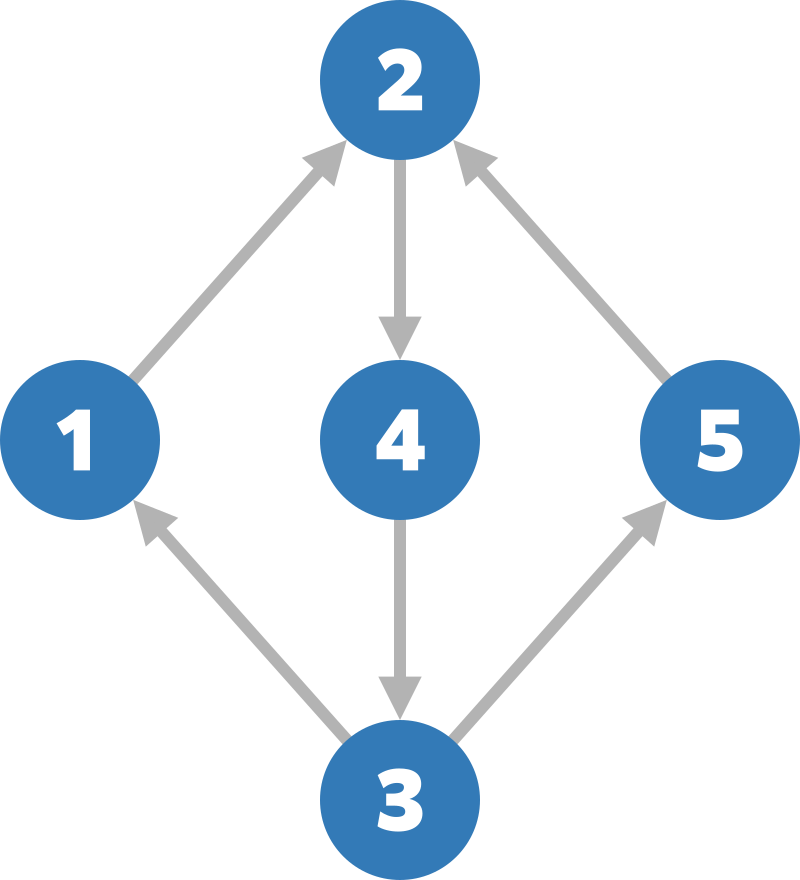
\includegraphics[width=0.5\linewidth]{flipEdge.png}
    \label{fig:enter-label}
\end{figure}

Você pode alcançar o vértice \(5\) com um custo total mínimo de \(4\) realizando, por exemplo, as seguintes operações:
\begin{itemize}
    \item Mova-se do vértice \(1\) para o vértice \(2\) (custo \(1\)).
    \item Mova-se do vértice \(2\) para o vértice \(4\) (custo \(1\)).
    \item Mova-se do vértice \(4\) para o vértice \(3\) (custo \(1\)).
    \item Mova-se do vértice \(3\) para o vértice \(5\) (custo \(1\)).
\end{itemize}

\subsubsection*{Solução}
A solução a seguir utiliza o algoritmo de Dijkstra aplicado a um estado ampliado que considera se as arestas estão no seu estado original ou invertido.

\begin{lstlisting}[language=C++]
void solve()
{
    int n, m, x; cin >> n >> m >> x;
    vvi graph(n+1), graph_inv(n+1);
    rep(i, 0, m){
        int x, y; cin >> x >> y;
        graph[x].pb(y);
        graph_inv[y].pb(x);
    }
    vvi dist(n+1, vi(2, LINF));

    priority_queue<tiii, vector<tiii>, greater<>> pq;
    dist[1][0] = 0;
    pq.push({0, 1, 0});
    while(pq.size()){
        auto [d, u, st] = pq.top(); pq.pop();
        if(dist[u][st] != d) continue;

        if(st == 0){
            for(auto v : graph[u]){
                if(dist[v][st] > d+1){
                    dist[v][st] = d+1;
                    pq.push({d+1, v, st});
                }
            }
        }else{
            for(auto v : graph_inv[u]){
                if(dist[v][st] > d+1){
                    dist[v][st] = d+1;
                    pq.push({d+1, v, st});
                }
            }
        }
        if(dist[u][1 - st] > d + x){
            dist[u][1 - st] = d + x;
            pq.push({dist[u][1-st], u, 1 - st});
        }
    }
    cout << min(dist[n][0], dist[n][1]) << endl;
}
\end{lstlisting}

\subsection{Audiophobia}

\subsubsection*{Enunciado}
Considere-se sortudo! Considere-se sortudo por ainda estar respirando e se divertindo participando deste concurso. Mas tememos que muitos de seus descendentes possam não ter esse privilégio. Pois, como você sabe, somos moradores de uma das cidades mais poluídas do mundo. A poluição está em toda parte, tanto no ambiente quanto na sociedade, e nossa falta de consciência só agrava a situação.

Por ora, porém, vamos considerar apenas um tipo de poluição – a poluição sonora. O nível de intensidade do som é geralmente medido em decibéis e sons com intensidade de 130 decibéis ou mais são considerados dolorosos. O nível de uma conversa normal é de 60 a 65 decibéis, enquanto o do tráfego intenso é de 70 a 80 decibéis.

Considere o seguinte mapa da cidade, onde as arestas representam ruas e os nós representam cruzamentos. O número inteiro em cada aresta indica o nível médio de intensidade sonora (em decibéis) na rua correspondente. Por exemplo, para ir do cruzamento A ao cruzamento G, você pode seguir o caminho A-C-F-G, o que exige tolerar um som de até 140 decibéis. Já para os caminhos A-B-E-G, A-B-D-G e A-C-F-D-G, é necessário tolerar, respectivamente, 90, 120 e 80 decibéis. Observa-se que o caminho A-C-F-D-G é o mais confortável, pois não demanda tolerância a mais de 80 decibéis.

Neste problema, dada a descrição do mapa da cidade, você deve determinar o nível mínimo de intensidade sonora (em decibéis) que você precisa tolerar para ir de um cruzamento a outro.

\subsubsection*{Entrada}
A entrada pode conter vários casos de teste. A primeira linha de cada caso de teste contém três inteiros \(C\), \(S\) e \(Q\), separados por espaços, onde:
\begin{itemize}
    \item \(C\) indica o número de cruzamentos (os cruzamentos são numerados de 1 a \(C\));
    \item \(S\) representa o número de ruas;
    \item \(Q\) é o número de consultas.
\end{itemize}
Cada uma das próximas \(S\) linhas contém três inteiros \(c_1\), \(c_2\) e \(d\), indicando que o nível médio de intensidade sonora na rua que conecta os cruzamentos \(c_1\) e \(c_2\) (com \(c_1 \neq c_2\)) é \(d\) decibéis.
Cada uma das próximas \(Q\) linhas contém dois inteiros \(c_1\) e \(c_2\) (\(c_1 \neq c_2\)), representando uma consulta: qual é o nível mínimo de intensidade sonora que você precisa tolerar para ir do cruzamento \(c_1\) para o cruzamento \(c_2\)?
A entrada termina com uma linha contendo três zeros separados por espaços.

\subsubsection*{Saída}
Para cada caso de teste, seu programa deve imprimir:
\begin{itemize}
    \item Primeiramente, o número do caso de teste (começando em 1) no formato “Case \#\(i\)”;
    \item Em seguida, para cada consulta, imprima uma linha contendo um inteiro, que é o nível mínimo de intensidade sonora (em decibéis) que deve ser tolerado para ir do primeiro ao segundo cruzamento da consulta. Se não existir um caminho entre eles, imprima “no path”.
\end{itemize}
Imprima uma linha em branco entre dois casos de teste consecutivos.

\subsubsection*{Exemplo de Entrada}
\begin{verbatim}
7 9 3
1 2 50
1 3 60
2 4 120
2 5 90
3 6 50
4 6 80
4 7 70
5 7 40
6 7 140
1 7
2 6
6 2
7 6 3
1 2 50
1 3 60
2 4 120
3 6 50
4 6 80
5 7 40
7 5
1 7
2 4
0 0 0
\end{verbatim}

\subsubsection*{Exemplo de Saída}
\begin{verbatim}
Case #1
80
60
60

Case #2
40
no path
80
\end{verbatim}



\begin{lstlisting}
int main()
{
    ios::sync_with_stdio(0);
    cin.tie(0);
    cout.tie(0);
    int n, m, q;
    int c = 0;
    while (cin >> n >> m >> q && (n || m || q))
    {
        vector<vector<int>> dist(n + 1, vector<int>(n + 1, INF));
        for (int i = 1; i <= n; i++)
        {
            dist[i][i] = 0;
        }

        for (int i = 0; i < m; i++)
        {
            int a, b, c;
            cin >> a >> b >> c;
            dist[a][b] = dist[b][a] = c;
        }

        for (int k = 1; k <= n; k++)
        {
            for (int i = 1; i <= n; i++)
            {
                for (int j = 1; j <= n; j++)
                {

                    dist[i][j] = min(dist[i][j], max(dist[i][k], dist[k][j]));
                }
            }
        }
        if(c) cout << endl ;
        cout << "Case #" << ++c << endl;
        while (q--)
        {
            int x, y;
            cin >> x >> y;
            ((dist[x][y] == INF) ? cout << "no path" : cout << dist[x][y]);

            cout << endl;
        }
    }
}
\end{lstlisting}
\newpage
\section{Dynamic Programming}
\subsection{Grid Paths}
Considere uma grade de \( n \times n \) cujos quadrados podem ter armadilhas. Não é permitido mover-se para um quadrado com armadilha. Sua tarefa é calcular o número de caminhos do quadrado superior esquerdo para o quadrado inferior direito, onde você só pode se mover para a direita ou para baixo.

Na primeira linha da entrada contém um inteiro \( n \): o tamanho da grade.  
Depois disso, há \( n \) linhas que descrevem a grade. Cada linha contém \( n \) caracteres:
\begin{itemize}
    \item \texttt{.} denota uma célula vazia;
    \item \texttt{*} denota uma armadilha.
\end{itemize}

\subsubsection*{Saída}
Imprima o número de caminhos possíveis, calculado módulo \( 10^9+7 \).

\subsubsection*{Restrições}
\[
1 \le n \le 1000
\]

\subsubsection*{Exemplo}

\textbf{Input:}
\begin{verbatim}
4
....
.*..
...*
*...
\end{verbatim}

\textbf{Output:}
\begin{verbatim}
3
\end{verbatim}

\subsubsection*{Solução}
\begin{lstlisting}[language=C++]
vector<vector<int>> DP;
vector<string> grid;
int N;

signed main()
{
    ios_base::sync_with_stdio(false);
    cin.tie(0);
    cout.tie(0);
    cin >> N;
    grid.resize(N);
    DP.assign(N, vector<int>(N, 0));
    DP[0][0] = 1;
    for (auto &i : grid)
        cin >> i;

    if(grid[0][0] == '*'){cout << 0 << endl; return 0;}
    for (int i = 0; i < N; i++)
    {
        for (int j = 0; j < N; j++)
        {
            if (grid[i][j] != '*')
            {
                if (i - 1 >= 0)
                    DP[i][j] += DP[i - 1][j];
                if (j - 1 >= 0)
                    DP[i][j] += DP[i][j - 1];
                DP[i][j] %= mod;
            }
        }
    }
    cout << DP[N - 1][N - 1] << endl;
}
\end{lstlisting}

\subsection{Coin Combinations I}
Considere um sistema monetário composto por \( n \) moedas. Cada moeda tem um valor inteiro positivo. Sua tarefa é calcular o número de maneiras distintas que você pode produzir uma soma de dinheiro \( x \) usando as moedas disponíveis.

Por exemplo, se as moedas forem \(\{2,3,5\}\) e a soma desejada for \(9\), existem \(8\) maneiras:
\begin{itemize}
    \item \(2+2+5\)
    \item \(2+5+2\)
    \item \(5+2+2\)
    \item \(3+3+3\)
    \item \(2+2+2+3\)
    \item \(2+2+3+2\)
    \item \(2+3+2+2\)
    \item \(3+2+2+2\)
\end{itemize}

\subsubsection*{Entrada}
A primeira linha da entrada contém dois inteiros \( n \) e \( x \): o número de moedas e a soma desejada, respectivamente.  
A segunda linha contém \( n \) inteiros distintos \( c_1, c_2, \dots, c_n \): o valor de cada moeda.

\subsubsection*{Saída}
Imprima um inteiro: o número de maneiras de produzir a soma \( x \) utilizando as moedas disponíveis, calculado módulo \( 10^9+7 \).

\subsubsection*{Restrições}
\[
1 \le n \le 100
\]
\[
1 \le x \le 10^6
\]
\[
1 \le c_i \le 10^6,\quad \text{para } i = 1, 2, \dots, n.
\]

\subsubsection*{Exemplo}

\textbf{Input:}
\begin{verbatim}
3 9
2 3 5
\end{verbatim}

\textbf{Output:}
\begin{verbatim}
8
\end{verbatim}

\subsubsection*{Solução}
\begin{lstlisting}[language=C++]
const int mod = 1000000007;

void solve() {
    int n, x;
    cin >> n >> x;
    vector<int> a(n);
    for(auto &coin : a)
        cin >> coin;
    
    vector<int> dp(x+1, 0);
    dp[0] = 1;
    
    for (int j = 1; j <= x; j++) {
        for (auto coin : a) {
            if (j - coin >= 0) {
                dp[j] += dp[j - coin];
                dp[j] %= mod;
            }
        }
    }
    
    cout << dp[x] << endl;
}

\end{lstlisting}

\subsection{Coin Combinations II}
Considere um sistema monetário composto por \( n \) moedas. Cada moeda tem um valor inteiro positivo. Sua tarefa é calcular o número de maneiras distintas \textbf{ordenadas} que você pode produzir uma soma de dinheiro \( x \) usando as moedas disponíveis.

Por exemplo, se as moedas forem \(\{2,3,5\}\) e a soma desejada for \(9\), existem \(3\) maneiras:
\begin{itemize}
    \item \(2+2+5\)
    \item \(3+3+3\)
    \item \(2+2+2+3\)
\end{itemize}

\subsubsection*{Entrada}
A primeira linha de entrada contém dois inteiros \( n \) e \( x \): o número de moedas e a soma desejada de dinheiro.\\  
A segunda linha contém \( n \) inteiros distintos \( c_1, c_2, \dots, c_n \): o valor de cada moeda.

\subsubsection*{Saída}
Imprima um inteiro: o número de maneiras módulo \( 10^9+7 \).

\subsubsection*{Restrições}
\[
1 \le n \le 100
\]
\[
1 \le x \le 10^6
\]
\[
1 \le c_i \le 10^6,\quad \text{para } i = 1, 2, \dots, n.
\]

\subsubsection*{Exemplo}

\textbf{Input:}
\begin{verbatim}
3 9
2 3 5
\end{verbatim}

\textbf{Output:}
\begin{verbatim}
3
\end{verbatim}

\subsubsection*{Solução}
\begin{lstlisting}[language=C++]
void solve()
{
    int n, v; 
    cin >> n >> v;
    vi a(n);
    for(auto &i : a) 
        cin >> i;

    vi dp(v+1, 0);
    dp[0] = 1;
    for(auto i : a){
        for(int j = i; j <= v; j++){
            dp[j] += dp[j - i];
            dp[j] %= mod;
        }
    }

    cout << dp[v] << endl;
}
\end{lstlisting}

\subsection{Dice Combinations}
Sua tarefa é contar o número de maneiras de construir a soma \( n \) jogando um dado uma ou mais vezes. Cada lançamento produz um resultado entre \( 1 \) e \( 6 \).

Por exemplo, se \( n = 3 \), existem \( 4 \) maneiras:
\begin{itemize}
    \item \(1+1+1\)
    \item \(1+2\)
    \item \(2+1\)
    \item \(3\)
\end{itemize}

\subsubsection*{Entrada}
A única linha de entrada contém um número inteiro \( n \).

\subsubsection*{Saída}
Imprima o número de maneiras de construir a soma \( n \) módulo \( 10^9+7 \).

\subsubsection*{Restrições}
\[
1 \le n \le 10^6
\]

\subsubsection*{Exemplo}

\textbf{Input:}
\begin{verbatim}
3
\end{verbatim}

\textbf{Output:}
\begin{verbatim}
4
\end{verbatim}

\subsubsection*{Solução}
\begin{lstlisting}[language=C++]
signed main()
{
    ios_base::sync_with_stdio(false);
    cin.tie(NULL);
    cout.tie(NULL);
    
    cin >> n;
    DP.assign(n + 1, 0);
    DP[0] = 1;
    
    for (int i = 1; i <= n; i++)
    {
        for (int j = 1; j <= 6; j++)
        {
            if (i - j >= 0)
            {
                DP[i] += DP[i - j];
                DP[i] %= mod;
            }
        }
    }
    cout << DP[n] << endl;
}
\end{lstlisting}

\subsection{Minimizing Coins}
Considere um sistema monetário composto por \( n \) moedas. Cada moeda tem um valor inteiro positivo. Sua tarefa é produzir uma quantia de dinheiro \( x \) usando as moedas disponíveis de forma que o número de moedas utilizado seja mínimo.

Por exemplo, se as moedas forem \(\{1,5,7\}\) e a quantia desejada for \(11\), uma solução ótima é \(5+5+1\), que utiliza \(3\) moedas.

\subsubsection*{Entrada}
A primeira linha de entrada contém dois inteiros \( n \) e \( x \): o número de moedas e a quantia desejada de dinheiro, respectivamente.\\  
A segunda linha contém \( n \) inteiros distintos \( c_1, c_2, \dots, c_n \): o valor de cada moeda.

\subsubsection*{Saída}
Imprima um inteiro: o número mínimo de moedas necessário para produzir a quantia \( x \). Se não for possível, imprima \(-1\).

\subsubsection*{Restrições}
\[
1 \le n \le 100
\]
\[
1 \le x \le 10^6
\]
\[
1 \le c_i \le 10^6,\quad \text{para } i = 1, 2, \dots, n.
\]

\subsubsection*{Exemplo}

\textbf{Input:}
\begin{verbatim}
3 11
1 5 7
\end{verbatim}

\textbf{Output:}
\begin{verbatim}
3
\end{verbatim}

\subsubsection*{Solução}
\begin{lstlisting}[language=C++]
int main()
{
    ios_base::sync_with_stdio(false);
    cin.tie(0);
    cout.tie(0);

    int n, x;
    cin >> n >> x;
    vector<int> dp(x + 1, inf);
    vector<int> moedas(n);

    for (auto &i : moedas)
        cin >> i;

    dp[0] = 0;

    for (int i = 1; i <= x; i++)
    {
        for (int j = 0; j < n; j++)
        {
            if (i - moedas[j] >= 0)
            {
                dp[i] = min(dp[i], dp[i - moedas[j]] + 1);
            }
        }
    }
    cout << (dp[x] == inf ? -1 : dp[x]) << endl;
    return 0;
}
\end{lstlisting}

\subsection{Removing Digits}
Você recebe um número inteiro \( n \). Em cada passo, você pode subtrair um dos dígitos (diferente de zero) do número. Sua tarefa é determinar o número mínimo de passos necessários para reduzir \( n \) a \( 0 \).

\subsubsection*{Entrada}
A única linha de entrada contém um número inteiro \( n \).

\subsubsection*{Saída}
Imprima um número inteiro: o número mínimo de passos necessários para transformar \( n \) em \( 0 \).

\subsubsection*{Restrições}
\[
1 \le n \le 10^6
\]

\subsubsection*{Exemplo}

\textbf{Input:}
\begin{verbatim}
27
\end{verbatim}

\textbf{Output:}
\begin{verbatim}
5
\end{verbatim}

\textbf{Explicação:} Uma solução ótima é: 
\[
27 \rightarrow 20 \rightarrow 18 \rightarrow 10 \rightarrow 9 \rightarrow 0
\]

\subsubsection*{Solução}
\begin{lstlisting}[language=C++]
int main() {
    int value;
    cin >> value;
    vector<int> dp(value + 1, INT_MAX);
    dp[0] = 0; // Não são necessárias operações para alcançar 0.

    for (int i = 1; i <= value; ++i) {
        int aux = i;
        while (aux > 0) {
            int digit = aux % 10;
            if (digit > 0) {
                dp[i] = min(dp[i], dp[i - digit] + 1);
            }
            aux /= 10;
        }
    }

    cout << dp[value] << endl;
    return 0;
}
\end{lstlisting}

\subsection{Book Shop}
Você está em uma livraria que vende \( n \) livros diferentes. Para cada livro, você sabe o seu preço e o número de páginas. Você decidiu que o preço total de suas compras será no máximo \( x \). Qual é o número máximo de páginas que você pode comprar? Note que você pode comprar cada livro no máximo uma vez.

\subsubsection*{Entrada}
A primeira linha da entrada contém dois inteiros \( n \) e \( x \): o número de livros e o preço total máximo.\\  
A próxima linha contém \( n \) inteiros \( h_1, h_2, \dots, h_n \): o preço de cada livro.\\  
A última linha contém \( n \) inteiros \( s_1, s_2, \dots, s_n \): o número de páginas de cada livro.

\subsubsection*{Saída}
Imprima um inteiro: o número máximo de páginas que você pode comprar.

\subsubsection*{Restrições}
\[
1 \le n \le 1000
\]
\[
1 \le x \le 10^5
\]
\[
1 \le h_i, s_i \le 1000
\]

\subsubsection*{Exemplo}

\textbf{Input:}
\begin{verbatim}
4 10
4 8 5 3
5 12 8 1
\end{verbatim}

\textbf{Output:}
\begin{verbatim}
13
\end{verbatim}

\textbf{Explicação:} Você pode comprar os livros 1 e 3. O preço total é \(4+5=9\) e o número total de páginas é \(5+8=13\).

\subsubsection*{Solução}
\begin{lstlisting}[language=C++]
int main(){
    int n, x;
    cin >> n >> x;
    vector<int> a(n), b(n), dp(x+1, 0);
    for(auto &i : a) 
        cin >> i;
    for(auto &i : b) 
        cin >> i;
    
    // dp[j] guarda o máximo de páginas que podemos obter com um custo total j
    for(int i = 0; i < n; i++){
        for(int j = x; j >= a[i]; j--){
            dp[j] = max(dp[j], dp[j - a[i]] + b[i]);
        }
    }
    cout << dp[x] << endl;
    return 0;
}
\end{lstlisting}

\subsection{Edit Distance}
Dada duas strings, a distância de edição é o número mínimo de operações necessárias para transformar uma string na outra. As operações permitidas são:
\begin{itemize}
    \item Adicionar um caractere à string;
    \item Remover um caractere da string;
    \item Substituir um caractere da string.
\end{itemize}

\subsubsection*{Entrada}
A primeira linha de entrada contém uma string com \( n \) caracteres (de A-Z).\\
A segunda linha de entrada contém uma string com \( m \) caracteres (de A-Z).

\subsubsection*{Saída}
Imprima um inteiro: a distância de edição entre as duas strings.

\subsubsection*{Restrições}
\[
1 \le n, m \le 5000
\]

\subsubsection*{Exemplo}

\textbf{Input:}
\begin{verbatim}
LOVE
MOVIE
\end{verbatim}

\textbf{Output:}
\begin{verbatim}
2
\end{verbatim}

\subsubsection*{Solução}
\begin{lstlisting}[language=C++]
void solve()
{
    string a, b;
    cin >> a >> b;
    int n = sz(a), m = sz(b);
    vvi dp(n + 1, vi(m + 1, 0));

    for (int i = 0; i <= n; i++) dp[i][0] = i;
    for (int j = 0; j <= m; j++) dp[0][j] = j;

    for (int i = 1; i <= n; i++)
    {
        for (int j = 1; j <= m; j++)
        {
            dp[i][j] = min({ dp[i - 1][j] + 1,
                             dp[i][j - 1] + 1,
                             dp[i - 1][j - 1] + (a[i - 1] != b[j - 1]) });
        }
    }
    cout << dp[n][m] << endl;
}
\end{lstlisting}

\subsection{Money Sums}
Você tem \( n \) moedas com certos valores. Sua tarefa é encontrar todas as somas de dinheiro que você pode criar usando essas moedas.

\subsubsection*{Entrada}
A primeira linha de entrada contém um inteiro \( n \): o número de moedas.\\
A segunda linha contém \( n \) inteiros \( x_1, x_2, \dots, x_n \): os valores das moedas.

\subsubsection*{Saída}
Primeiro, imprima um inteiro \( k \): o número de somas de dinheiro distintas (exceto 0). Após isso, imprima todas as somas possíveis em ordem crescente, separadas por um espaço.

\subsubsection*{Restrições}
\[
1 \le n \le 100,\quad 1 \le x_i \le 1000
\]

\subsubsection*{Exemplo}

\textbf{Input:}
\begin{verbatim}
4
4 2 5 2
\end{verbatim}

\textbf{Output:}
\begin{verbatim}
9
2 4 5 6 7 8 9 11 13
\end{verbatim}

\subsubsection*{Solução}
\begin{lstlisting}[language=C++]
void solve()
{
    int n; 
    cin >> n;
    vi a(n);
    for(auto &i : a) 
        cin >> i;
    set<int> ans = {0};
    for(auto i : a){
        set<int> st;
        for(auto j : ans){
            st.insert(j + i);
        }
        ans.insert(st.begin(), st.end());
    }
    cout << ans.size() - 1 << endl;
    for(auto i : ans){
        if(i == 0) continue;
        cout << i << " ";
    }
    cout << endl;
}
\end{lstlisting}

\subsection{Rectangle Cutting}
Dado um retângulo de \( a \times b \), sua tarefa é cortá-lo em quadrados. Em cada movimento, você pode selecionar um retângulo e cortá-lo em dois retângulos de forma que todos os comprimentos dos lados permaneçam inteiros. Qual é o número mínimo de movimentos necessários?

\subsubsection*{Entrada}
A única linha de entrada contém dois inteiros \( a \) e \( b \): as dimensões do retângulo.

\subsubsection*{Saída}
Imprima um inteiro: o número mínimo de movimentos.

\subsubsection*{Restrições}
\[
1 \le a, b \le 500
\]

\subsubsection*{Exemplo}

\textbf{Input:}
\begin{verbatim}
3 5
\end{verbatim}

\textbf{Output:}
\begin{verbatim}
3
\end{verbatim}

\subsubsection*{Solução}
\begin{lstlisting}[language=C++]
void solve()
{
    int a, b;
    cin >> a >> b;
    vvi dp(a + 1, vi(b + 1, INF));

    rep(i, 1, a + 1)
    {
        rep(j, 1, b + 1)
        {
            if (i == j)
            {
                dp[i][j] = 0;
                continue;
            }
            rep(k, 1, i)
            {
                dp[i][j] = min(dp[i][j], dp[k][j] + dp[i - k][j] + 1);
            }
            rep(k, 1, j)
            {
                dp[i][j] = min(dp[i][j], dp[i][k] + dp[i][j - k] + 1);
            }
        }
    }
    cout << dp[a][b] << endl;
}
\end{lstlisting}

\subsection{Array Description}
Dado que um array possui \( n \) inteiros entre \( 1 \) e \( m \), e a diferença absoluta entre dois valores adjacentes é no máximo \( 1 \), dada uma descrição do array onde alguns valores podem ser desconhecidos (representados por \( 0 \)), sua tarefa é contar o número de arrays que correspondem à descrição.

\subsubsection*{Entrada}
A primeira linha de entrada contém dois inteiros \( n \) e \( m \): o tamanho do array e o limite superior para cada valor.\\
A próxima linha contém \( n \) inteiros \( x_1, x_2, \dots, x_n \): o conteúdo do array. O valor \( 0 \) denota um valor desconhecido.

\subsubsection*{Saída}
Imprima um inteiro: o número de arrays que correspondem à descrição, módulo \( 10^9+7 \).

\subsubsection*{Restrições}
\[
1 \le n \le 10^5,\quad 1 \le m \le 100,\quad 0 \le x_i \le m
\]

\subsubsection*{Exemplo}

\textbf{Input:}
\begin{verbatim}
3 5
2 0 2
\end{verbatim}

\textbf{Output:}
\begin{verbatim}
3
\end{verbatim}

\subsubsection*{Solução}
\begin{lstlisting}[language=C++]
void solve()
{
    int n, m;
    cin >> n >> m;
    vi a(n);
    for (auto &i : a)
        cin >> i;

    vvi dp(n, vi(m + 1, 0));
    if(a[0] == 0)
        for (int i = 1; i <= m; i++)
            dp[0][i] = 1;
    else dp[0][a[0]] = 1;

    for (int i = 1; i < n; i++)
    {
        if (a[i] == 0)
        {
            for (int j = 1; j <= m; j++)
            {
                dp[i][j] = dp[i - 1][j];
                if (j > 1)
                {
                    dp[i][j] += dp[i - 1][j - 1];
                    dp[i][j] %= mod;
                }
                if (j < m)
                {
                    dp[i][j] += dp[i - 1][j + 1];
                    dp[i][j] %= mod;
                }
            }
        }
        else
        {
            dp[i][a[i]] = dp[i - 1][a[i]];
            if (a[i] > 1)
            {
                dp[i][a[i]] += dp[i - 1][a[i] - 1];
                dp[i][a[i]] %= mod;
            }
            if (a[i] < m)
            {
                dp[i][a[i]] += dp[i - 1][a[i] + 1];
                dp[i][a[i]] %= mod;
            }
        }
    }
    int ans = 0;
    for (int i = 1; i <= m; i++)
    {
        ans += dp[n-1][i];
        ans %= mod;
    }
    cout << ans << endl;
}
\end{lstlisting}
\subsection{Increasing Subsequence}
Dado um array de \( n \) inteiros, sua tarefa é determinar o comprimento da subsequência crescente mais longa, ou seja, a subsequência de elementos que é estritamente crescente e possui o maior tamanho possível. Uma subsequência é uma sequência que pode ser derivada do array removendo alguns elementos sem alterar a ordem dos elementos restantes.

\subsubsection*{Entrada}
A primeira linha contém um inteiro \( n \): o tamanho do array.\\
A segunda linha contém \( n \) inteiros \( x_1, x_2, \dots, x_n \): o conteúdo do array.

\subsubsection*{Saída}
Imprima o comprimento da subsequência crescente mais longa.

\subsubsection*{Restrições}
\[
1 \le n \le 2\cdot 10^5,\quad 1 \le x_i \le 10^9
\]

\subsubsection*{Exemplo}

\textbf{Input:}
\begin{verbatim}
8
7 3 5 3 6 2 9 8
\end{verbatim}

\textbf{Output:}
\begin{verbatim}
4
\end{verbatim}

\subsubsection*{Solução}
\begin{lstlisting}[language=C++]
void solve()
{
    int n; 
    cin >> n;
    vi v(n);
    for(auto &i : v) 
        cin >> i;
    vi ans;
    for(int i = 0; i < n; i++){
        auto it = lower_bound(all(ans), v[i]);
        if(it == ans.end()) 
            ans.pb(v[i]);
        else 
            *it = v[i];
    }
    cout << ans.size() << endl;
}
\end{lstlisting}

\subsection{Projects}
Você tem \( n \) projetos aos quais pode comparecer. Para cada projeto, você sabe o dia de início \( a_i \), o dia de término \( b_i \) e a recompensa \( p_i \). Você só pode comparecer a um projeto por dia, ou seja, os projetos escolhidos não podem se sobrepor. Sua tarefa é determinar a quantidade máxima de dinheiro que você pode ganhar escolhendo um conjunto de projetos compatível.

\subsubsection*{Entrada}
A primeira linha de entrada contém um inteiro \( n \): o número de projetos.\\
Em seguida, há \( n \) linhas, cada uma contendo três inteiros \( a_i \), \( b_i \) e \( p_i \), representando, respectivamente, o dia de início, o dia de término e a recompensa do projeto.

\subsubsection*{Saída}
Imprima um inteiro: a quantidade máxima de dinheiro que você pode ganhar.

\subsubsection*{Restrições}
\[
1 \le n \le 2 \cdot 10^5,\quad 1 \le a_i \le b_i \le 10^9,\quad 1 \le p_i \le 10^9.
\]

\subsubsection*{Exemplo}

\textbf{Input:}
\begin{verbatim}
4
2 4 4
3 6 6
6 8 2
5 7 3
\end{verbatim}

\textbf{Output:}
\begin{verbatim}
7
\end{verbatim}

\subsubsection*{Solução}
\begin{lstlisting}[language=C++]
struct project {
    int start, end, reward;
};

void solve()
{
    int n;
    cin >> n;
    vector<project> projects(n);
    for (auto &i : projects)
    {
        cin >> i.start >> i.end >> i.reward;
    }
    sort(all(projects), [&](project a, project b)
         { return a.end < b.end; });
    vi dp(n, 0);
    dp[0] = projects[0].reward;

    for (int i = 1; i < n; i++)
    {
        int l = -1, r = i - 1;
        while (l != r)
        {
            int m = (l + r + 1) / 2;
            if (projects[m].end < projects[i].start)
                l = m;
            else
                r = m - 1;
        }
        if (l != -1)
            dp[i] = max(dp[i - 1], projects[i].reward + dp[l]);
        else
            dp[i] = max(dp[i - 1], projects[i].reward);
    }
    cout << dp[n - 1] << endl;
}
\end{lstlisting}
\subsection{Counting Tilings}
Sua tarefa é contar o número de maneiras de preencher uma grade de \( n \times m \) usando azulejos de \(1 \times 2\) e \(2 \times 1\).

\subsubsection*{Entrada}
A única linha de entrada contém dois inteiros \( n \) e \( m \).

\subsubsection*{Saída}
Imprima um inteiro: o número de maneiras de preencher a grade, módulo \(10^9+7\).

\subsubsection*{Restrições}
\[
1 \le n \le 10,\quad 1 \le m \le 1000.
\]

\subsubsection*{Exemplo}

\textbf{Input:}
\begin{verbatim}
4 7
\end{verbatim}

\textbf{Output:}
\begin{verbatim}
781
\end{verbatim}

\subsubsection*{Solução}
\begin{lstlisting}[language=C++]
void solve()
{
    int n, m;
    cin >> n >> m;
    vvi dp(m+1, vi(1 << n, 0));
    dp[0][0] = 1;
    rep(i, 0, m) {
        rep(mask, 0, 1 << n) {
            auto fillColumn = [&](auto &fillColumn, int pos, int curr_mask, int next_mask) -> void {
                if(pos == n) {
                    dp[i+1][next_mask] = (dp[i+1][next_mask] + dp[i][mask]) % mod;
                    return;
                }
                if(curr_mask & (1 << pos)) {
                    fillColumn(fillColumn, pos+1, curr_mask, next_mask);
                } else {
                    // Tenta colocar um domino vertical (afeta apenas a coluna atual)
                    if(pos+1 < n && !(curr_mask & (1 << (pos+1))))
                        fillColumn(fillColumn, pos+2, curr_mask, next_mask);
                    // Tenta colocar um domino horizontal (preenche a célula da próxima coluna)
                    fillColumn(fillColumn, pos+1, curr_mask, next_mask | (1 << pos));
                }
            };
            fillColumn(fillColumn, 0, mask, 0);
        }
    }
    cout << dp[m][0] << endl;
}
\end{lstlisting}

\subsection{Two Sets II}
Dada a sequência dos números \(1,2,\ldots,n\), sua tarefa é contar o número de maneiras de dividi-la em dois conjuntos cuja soma seja igual.

\subsubsection*{Entrada}
A única linha de entrada contém um inteiro \(n\).

\subsubsection*{Saída}
Imprima um inteiro: o número de maneiras de dividir os números de \(1\) a \(n\) em dois conjuntos de soma igual, módulo \(10^9+7\).

\subsubsection*{Restrições}
\[
1 \le n \le 500
\]

\subsubsection*{Exemplo}

\textbf{Input:}
\begin{verbatim}
7
\end{verbatim}

\textbf{Output:}
\begin{verbatim}
4
\end{verbatim}

\subsubsection*{Solução}
\begin{lstlisting}[language=C++]
void solve()
{
    int n; 
    cin >> n;
    int sum = n * (n + 1) / 2;
    if (sum & 1) {
        cout << 0 << endl;
        return;
    }
    int target = sum / 2;
    vi dp(MAXN);
    dp[0] = 1;
    rep(i, 1, n+1){
        for (int j = i*(i-1)/2; j >= 0; j--){
            dp[j+i] = (dp[j+i] + dp[j]) % (2 * mod);
        }
    }
    cout << dp[target] / 2 << endl;
}
\end{lstlisting}
\subsection{Unique Paths}
Há um robô em uma grade de tamanho \( m \times n \). O robô está inicialmente localizado no \textbf{canto superior esquerdo} (ou seja, em \texttt{grid[0][0]}). O robô tenta se mover para o \textbf{canto inferior direito} (ou seja, em \texttt{grid[m-1][n-1]}). Em cada movimento, ele pode apenas se mover para \textbf{baixo} ou para \textbf{direita}.

Dado os dois inteiros \( m \) e \( n \), retorne o número de caminhos únicos possíveis que o robô pode seguir para alcançar o canto inferior direito. Os casos de teste são gerados de forma que a resposta seja menor ou igual a \(2 \times 10^9\).

\subsubsection*{Entrada}
A única linha de entrada contém dois inteiros \( m \) e \( n \).

\subsubsection*{Saída}
Imprima um inteiro: o número de caminhos únicos.

\subsubsection*{Restrições}
\[
1 \le m, n \le 100
\]

\subsubsection*{Exemplo}

\textbf{Exemplo 1:}

\textbf{Input:}
\begin{verbatim}
3 7
\end{verbatim}

\textbf{Output:}
\begin{verbatim}
28
\end{verbatim}

\textbf{Exemplo 2:}

\textbf{Input:}
\begin{verbatim}
3 2
\end{verbatim}

\textbf{Output:}
\begin{verbatim}
3
\end{verbatim}

\subsubsection*{Solução}
\begin{lstlisting}[language=C++]
int uniquePaths(int m, int n) {
    vvi dp(m, vi(n, 0));
    dp[0][0] = 1;
    for (int i = 0; i < m; i++) {
        for (int j = 0; j < n; j++) {
            if (i > 0)
                dp[i][j] += dp[i-1][j];
            if (j > 0)
                dp[i][j] += dp[i][j-1];
        }
    }
    return dp[m-1][n-1];
}
\end{lstlisting}
\subsection{Maximal Square}
Dada uma matriz binária \(m \times n\) preenchida com os caracteres \texttt{'0'} e \texttt{'1'}, sua tarefa é encontrar o maior quadrado que contenha apenas \texttt{'1'} e retornar sua área.

\subsubsection*{Entrada}
A entrada consiste em uma matriz binária, onde:
\begin{itemize}
    \item \(m = \texttt{matrix.length}\)
    \item \(n = \texttt{matrix[i].length}\)
\end{itemize}

\subsubsection*{Saída}
Imprima um inteiro: a área do maior quadrado formado apenas por \texttt{'1'}.

\subsubsection*{Restrições}
\[
1 \le m, n \le 300.
\]

\subsubsection*{Exemplo}

\textbf{Input:}
\begin{verbatim}
[["1","0","1","0","0"],
 ["1","0","1","1","1"],
 ["1","1","1","1","1"],
 ["1","0","0","1","0"]]
\end{verbatim}

\textbf{Output:}
\begin{verbatim}
4
\end{verbatim}

\subsubsection*{Solução}
\begin{lstlisting}[language=C++]
int maximalSquare(vector<vector<char>>& matrix) {
    if (matrix.empty() || matrix[0].empty()) return 0;
    int m = matrix.size(), n = matrix[0].size();
    vector<vector<int>> dp(m, vector<int>(n, 0));
    int maxSide = 0;

    for (int i = 0; i < m; ++i) {
        for (int j = 0; j < n; ++j) {
            if (matrix[i][j] == '1') {
                if (i == 0 || j == 0)
                    dp[i][j] = 1;
                else
                    dp[i][j] = min({dp[i-1][j], dp[i][j-1], dp[i-1][j-1]}) + 1;
                maxSide = max(maxSide, dp[i][j]);
            }
        }
    }
    return maxSide * maxSide;
}
\end{lstlisting}

\subsection{Mínimas Inserções para Formar um Palíndromo}

Dada uma string \( s \), em um único passo você pode inserir qualquer caractere em qualquer índice da string.

Retorne o \textit{número mínimo de passos} necessários para transformar \( s \) em um palíndromo.

\subsubsection*{Definição}
Uma string palindrômica é aquela que pode ser lida da mesma forma tanto da esquerda para a direita quanto da direita para a esquerda.

\subsubsection*{Entrada}
A entrada consiste em uma única string \( s \) contendo apenas letras minúsculas do alfabeto inglês.

\subsubsection*{Saída}
Imprima um inteiro representando o número mínimo de inserções para tornar a string um palíndromo.

\subsubsection*{Restrições}
\[
1 \leq \text{s.length} \leq 500
\]

\subsubsection*{Exemplo}

\textbf{Entrada:}
\begin{verbatim}
s = "zzazz"
\end{verbatim}

\textbf{Saída:}
\begin{verbatim}
0
\end{verbatim}

\textbf{Explicação:} A string \texttt{"zzazz"} já é um palíndromo, então não é necessário fazer nenhuma inserção.

\bigskip
\textbf{Entrada:}
\begin{verbatim}
s = "mbadm"
\end{verbatim}

\textbf{Saída:}
\begin{verbatim}
2
\end{verbatim}

\textbf{Explicação:} Podemos formar os palíndromos \texttt{"mbdadbm"} ou \texttt{"mdbabdm"} com duas inserções.

\bigskip
\textbf{Entrada:}
\begin{verbatim}
s = "leetcode"
\end{verbatim}

\textbf{Saída:}
\begin{verbatim}
5
\end{verbatim}

\textbf{Explicação:} Inserindo 5 caracteres, a string pode se tornar \texttt{"leetcodocteel"}.

\subsubsection*{Solução}
\begin{lstlisting}[language=C++]
int minInsertions(string s) {
    int n = s.size();
    vector<vector<int>> dp(n + 1, vector<int>(n + 1));

    for (int i = 0; i <= n; i++)
        dp[i][i] = 1;

    for (int i = n - 2; i >= 0; i--) {
        for (int j = i + 1; j < n; j++) {
            if (s[i] == s[j]) {
                dp[i][j] = dp[i + 1][j - 1] + 2;
            } else {
                dp[i][j] = max(dp[i + 1][j], dp[i][j - 1]);
            }
        }
    }
    return n - dp[0][n - 1];
}
\end{lstlisting}

\subsection{Subsequência Comum Mais Longa}

Dadas duas strings \( \text{text1} \) e \( \text{text2} \), retorne o comprimento de sua \textbf{subsequência comum mais longa}. Se não houver subsequência comum, retorne \( 0 \).

\subsubsection*{Definição}
Uma \textbf{subsequência} de uma string é uma nova string gerada a partir da string original ao remover alguns caracteres (ou nenhum), sem alterar a ordem relativa dos caracteres restantes.

Por exemplo, \texttt{"ace"} é uma subsequência de \texttt{"abcde"}.

Uma \textbf{subsequência comum} de duas strings é uma subsequência que aparece em ambas.

\subsubsection*{Entrada}
A entrada consiste em duas strings \( \text{text1} \) e \( \text{text2} \), contendo apenas letras minúsculas do alfabeto inglês.

\subsubsection*{Saída}
Imprima um inteiro representando o comprimento da maior subsequência comum entre as duas strings.

\subsubsection*{Restrições}
\[
1 \leq \text{text1.length}, \text{text2.length} \leq 1000
\]

\subsubsection*{Exemplo}

\textbf{Entrada:}
\begin{verbatim}
text1 = "abcde", text2 = "ace"
\end{verbatim}

\textbf{Saída:}
\begin{verbatim}
3
\end{verbatim}

\textbf{Explicação:} A subsequência comum mais longa é \texttt{"ace"}, que possui comprimento 3.

\bigskip
\textbf{Entrada:}
\begin{verbatim}
text1 = "abc", text2 = "abc"
\end{verbatim}

\textbf{Saída:}
\begin{verbatim}
3
\end{verbatim}

\textbf{Explicação:} A subsequência comum mais longa é \texttt{"abc"}, que possui comprimento 3.

\bigskip
\textbf{Entrada:}
\begin{verbatim}
text1 = "abc", text2 = "def"
\end{verbatim}

\textbf{Saída:}
\begin{verbatim}
0
\end{verbatim}

\textbf{Explicação:} Não há subsequência comum entre as strings, então o resultado é 0.

\subsubsection*{Solução}
\begin{lstlisting}[language=C++]
int longestCommonSubsequence(string text1, string text2) {
    int m = text1.size();
    int n = text2.size();
    vector<vector<int>> dp(2, vector<int>(n + 1, 0)); // duas linhas apenas

    for (int i = 1; i <= m; i++) {
        for (int j = 1; j <= n; j++) {
            if (text1[i - 1] == text2[j - 1]) {
                dp[i % 2][j] = 1 + dp[(i - 1) % 2][j - 1];
            } else {
                dp[i % 2][j] = max(dp[(i - 1) % 2][j], dp[i % 2][j - 1]);
            }
        }
    }

    return dp[m % 2][n];
}
\end{lstlisting}


\newpage
\section{Ordered Set}
\subsection{List Removals}

\subsubsection*{Enunciado}
Você recebe uma lista composta por \( n \) inteiros. Sua tarefa é remover elementos da lista em posições dadas e relatar os elementos removidos.

\subsubsection*{Entrada}
A primeira linha de entrada contém um inteiro \( n \): o tamanho inicial da lista. Durante o processo, os elementos são numerados \( 1, 2, \dots, k \), onde \( k \) é o tamanho atual da lista.

A segunda linha contém \( n \) inteiros \( x_1, x_2, \dots, x_n \): o conteúdo da lista.

A última linha contém \( n \) inteiros \( p_1, p_2, \dots, p_n \): as posições dos elementos a serem removidos.

\subsubsection*{Saída}
Imprima os elementos na ordem em que foram removidos.

\subsubsection*{Restrições}
\[
1 \le n \le 2 \cdot 10^5
\]
\[
1 \le x_i \le 10^9
\]
\[
1 \le p_i \le n - i + 1
\]

\subsubsection*{Solução}
\begin{lstlisting}[language=C++]
void solve()
{
    int n; cin >> n;
    vi a(n);
    ordered_set<int> s;
    rep(i, 0, n){
        cin >> a[i];
        s.insert(i);
    }
    rep(i, 0, n){
        int p; cin >> p;
        int pos = *s.find_by_order(p-1);
        cout << a[pos] << " ";
        s.erase(pos);
    }
}
\end{lstlisting}


\subsection{Poblema 2}

\subsubsection*{Enunciado}
Você recebe um array de \( n \) inteiros. Sua tarefa é calcular a mediana de cada janela de \( k \) elementos, da esquerda para a direita.

A mediana é o elemento do meio quando os elementos estão ordenados. Se o número de elementos for par, existem duas medianas possíveis e assumimos que a mediana é a menor delas.

\subsubsection*{Entrada}
A primeira linha contém dois inteiros \( n \) e \( k \): o número de elementos e o tamanho da janela.

Em seguida, há \( n \) inteiros \( x_1, x_2, \dots, x_n \): o conteúdo do array.

\subsubsection*{Saída}
Imprima \( n-k+1 \) valores: as medianas.

\subsubsection*{Restrições}
\[
1 \le k \le n \le 2 \cdot 10^5
\]
\[
1 \le x_i \le 10^9, \quad \text{para } i = 1, 2, \dots, n.
\]


\subsubsection*{Solução}
\begin{lstlisting}[language=C++]
void solve()
{
    int n, k; cin >> n >> k;
    vi a(n);
    ordered_set<pii> s;
    rep(i, 0, n){
        cin >> a[i];
        if(i < k) // Insere apenas os primeiros k elementos.
            s.insert({a[i], i});
    }
    // a mediana será o elemento 
    // na posição (k-1)/2 (0-indexed)
    auto med = s.find_by_order((k-1)/2);
    cout << med->f << ' ';
    rep(i, k, n){
        // Insere o novo elemento com seu índice.
        s.insert({a[i], i});
        // Remove o elemento que saiu da janela.
        s.erase(s.find({a[i-k], i-k}));
        // Busca a mediana da janela atual.
        med = s.find_by_order((k-1)/2);
        cout << med->f << ' ';
    }
    cout << endl;
}
    
\end{lstlisting}

\newpage
\section{Fenwick}
\subsection{Rotated Inversions}

\subsubsection*{Enunciado}
Você recebe inteiros \(N, M\) e uma sequência de inteiros não negativos de comprimento \(N\):
\[
A = (A_1, A_2, \ldots, A_N).
\]
Para cada inteiro \(k\) com \(0 \le k \le M-1\), defina a sequência
\[
B = (B_1, B_2, \ldots, B_N),
\]
onde
\[
B_i = (A_i + k) \bmod M.
\]
Sua tarefa é calcular o número de inversões na sequência \(B\). O número de inversões de uma sequência é o número de pares \((i,j)\) tais que
\[
1 \le i < j \le N \quad \text{e} \quad B_i > B_j.
\]

\subsubsection*{Restrições}
\begin{itemize}
    \item \(1 \le N, M \le 2 \times 10^5\).
    \item \(0 \le A_i < M\) para \(1 \le i \le N\).
    \item Todos os valores de entrada são inteiros.
\end{itemize}

\subsubsection*{Entrada}
A entrada é fornecida a partir da entrada padrão no seguinte formato:
\begin{verbatim}
N M
A_1 A_2 \dots A_N
\end{verbatim}

\subsubsection*{Saída}
Imprima \(M\) linhas. A \(i\)-ésima linha (para \(1 \le i \le M\)) deve conter a resposta para o caso \(k = i-1\); isto é, o número de inversões na sequência \(B\) formada com \(k = i-1\).

\subsubsection*{Exemplo 1}
\textbf{Entrada:}
\begin{verbatim}
3 3
2 1 0
\end{verbatim}
\textbf{Saída:}
\begin{verbatim}
3
1
1
\end{verbatim}

\subsubsection*{Exemplo 2}
\textbf{Entrada:}
\begin{verbatim}
5 6
5 3 5 0 1
\end{verbatim}
\textbf{Saída:}
\begin{verbatim}
7
3
3
1
1
5
\end{verbatim}

\subsubsection*{Exemplo 3}
\textbf{Entrada:}
\begin{verbatim}
7 7
0 1 2 3 4 5 6
\end{verbatim}
\textbf{Saída:}
\begin{verbatim}
0
6
10
12
12
10
6
\end{verbatim}

\subsubsection*{Solução}
A seguir, uma possível solução em C++ que utiliza uma Árvore de Fenwick (BIT) para contar inversões e aproveita o fato de que as inversões podem ser atualizadas de forma incremental ao rotacionar a sequência.

\begin{lstlisting}[language=C++]
class FenwickTree {
    private:
        int n;
        vector<int> tree;
    public:
        // Cria uma BIT com n posições (0-indexado publicamente)
        FenwickTree(int n) : n(n), tree(n+1, 0) {}

        // Adiciona 'x' na posição p (0-indexada)
        void add(int p, int x) {
            for(++p; p <= n; p += p & -p)
                tree[p] += x;
        }

        // Soma prefixo [0, p)
        int sum(int p) const {
            int res = 0;
            for(; p; p -= p & -p)
                res += tree[p];
            return res;
        }

        // Soma no intervalo [l, r)
        int range_sum(int l, int r) const {
            return sum(r) - sum(l);
        }
};

void solve()
{
    int n, m;
    cin >> n >> m;
    // Para cada valor de A, armazena os índices onde ele ocorre.
    vector<vector<int>> g(m);
    vector<int> a(n);
    for (int i = 0; i < n; i++){
        cin >> a[i];
        g[a[i]].push_back(i);
    }
    
    int ans = 0;
    FenwickTree fenw(m);
    // Contagem de inversões na sequencia A (caso k = 0)
    for (auto x : a) {
        ans += fenw.range_sum(x + 1, m);
        fenw.add(x, 1);
    }
    cout << ans << endl;
    
    // Para cada rotação k de 1 a m-1, atualize o número de inversões
    for (int c = 1; c < m; c++){
        int c1 = 0, c2 = 0;
        // 'g[m-c]' armazena os índices dos elementos iguais a m-c
        auto &grupo = g[m - c];
        for (int i = 0; i < (int)grupo.size(); i++){
            c1 += grupo[i] - i;
            c2 += (n - 1 - grupo[i]) - ((int)grupo.size() - 1 - i);
        }
        ans += c1 - c2;
        cout << ans << endl;
    }
}
\end{lstlisting}

\subsection{Insert}

\subsubsection*{Enunciado}
Há um array vazio \(A\). Para \(i = 1, 2, \dots, N\), execute a seguinte operação em ordem:
\begin{itemize}
    \item Insira o número \(i\) em \(A\) de modo que se torne o \(P_i\)-ésimo elemento a partir do início.
    \begin{itemize}
        \item Mais precisamente, substitua \(A\) pela concatenação dos primeiros \(P_i - 1\) elementos de \(A\), seguido por \(i\), e depois os elementos restantes de \(A\) a partir do \(P_i\)-ésimo elemento, nesta ordem.
    \end{itemize}
\end{itemize}
Ao final, obtenha o array final \(A\).

\subsubsection*{Restrições}
\[
1 \leq N \leq 5 \times 10^5
\]
\[
1 \leq P_i \leq i \quad \text{para } i = 1, 2, \dots, N.
\]
Todos os valores de entrada são inteiros.

\subsubsection*{Entrada}
A entrada é fornecida a partir da entrada padrão no seguinte formato:
\begin{verbatim}
N
P_1 P_2 ... P_N
\end{verbatim}

\subsubsection*{Saída}
Seja o array final 
\[
A = (A_1, A_2, \dots, A_N).
\]
Imprima \(A_1, A_2, \dots, A_N\) nesta ordem, separados por espaços.

\subsubsection*{Exemplo 1}
\textbf{Input:}
\begin{verbatim}
4
1 1 2 1
\end{verbatim}

\textbf{Output:}
\begin{verbatim}
4 2 3 1
\end{verbatim}

\textbf{Explicação:}
\begin{enumerate}
    \item Insira o número \(1\) de modo que se torne o 1º elemento de \(A\). Agora, \(A = (1)\).
    \item Insira o número \(2\) de modo que se torne o 1º elemento de \(A\). Agora, \(A = (2, 1)\).
    \item Insira o número \(3\) de modo que se torne o 2º elemento de \(A\). Agora, \(A = (2, 3, 1)\).
    \item Insira o número \(4\) de modo que se torne o 1º elemento de \(A\). Agora, \(A = (4, 2, 3, 1)\).
\end{enumerate}

\subsubsection*{Exemplo 2}
\textbf{Input:}
\begin{verbatim}
5
1 2 3 4 5
\end{verbatim}

\textbf{Output:}
\begin{verbatim}
1 2 3 4 5
\end{verbatim}


\begin{lstlisting}
    struct BIT {
    int n;
    vector<int> tree;
    BIT(int n): n(n), tree(n+1, 0) {}

    void update(int idx, int delta) {
        for(; idx <= n; idx += idx & -idx)
            tree[idx] += delta;
    }

    int query(int idx) {
        int sum = 0;
        for(; idx; idx -= idx & -idx)
            sum += tree[idx];
        return sum;
    }

    int find(int k) {
        int idx = 0;
        for (int bit = 1 << 20; bit; bit >>= 1) {
            int next = idx + bit;
            if(next <= n && tree[next] < k) {
                k -= tree[next];
                idx = next;
            }
        }
        return idx+1;
    }
};

void solve() {
    int n;
    cin >> n;
    vi p(n), a(n+1, 0);
    for (auto &x : p) cin >> x;

    BIT bit(n);
    rep (i, 1, n+1)
        bit.update(i, 1);


    for(int i = n; i >= 1; i--) {
        int pos = bit.find(p[i-1]);
        a[pos] = i;
        bit.update(pos, -1);
    }

    rep(i,1,n+1){
        cout << a[i] << " ";
    }
    cout << endl;
}
\end{lstlisting}
\newpage
\section{Busca Binaria}

\subsection{Smooth Occlusion}

\subsubsection*{Enunciado}
Takahashi tem \(2N\) dentes: \(N\) dentes superiores e \(N\) dentes inferiores.
O comprimento do \(i\)-ésimo dente superior da esquerda é \(U_i\) e o do \(i\)-ésimo dente inferior da esquerda é \(D_i\) (para \(1 \le i \le N\)).
Os dentes estão considerados "bem ajustados" se ambas as seguintes condições forem satisfeitas:
\begin{enumerate}
    \item Existe um inteiro \(H\) tal que, para todo \(i\) com \(1 \le i \le N\),
    \[
    U_i + D_i = H.
    \]
    \item Para todo \(i\) com \(1 \le i < N\),
    \[
    \lvert U_i - U_{i+1} \rvert \le X.
    \]
\end{enumerate}

Takahashi não pode aumentar os comprimentos dos dentes, apenas reduzi-los.
Para isso, ele dispõe de uma máquina de moagem de dentes: a cada operação, pagando 1 iene, ele pode escolher exatamente um dente cujo comprimento seja positivo e reduzir seu comprimento em 1.
Encontre o valor total mínimo que ele precisa pagar para que seus dentes se ajustem bem.

\subsubsection*{Restrições}
\begin{itemize}
    \item \(2 \le N \le 2 \times 10^5\).
    \item \(1 \le X \le 10^9\).
    \item \(1 \le U_i, D_i \le 10^9\) para \(1 \le i \le N\).
\end{itemize}

\subsubsection*{Entrada}
A entrada é fornecida a partir da entrada padrão no seguinte formato:
\begin{verbatim}
N X
U_1 D_1
U_2 D_2
.
.
.
U_N D_N
\end{verbatim}

\subsubsection*{Saída}
Imprima uma única linha contendo o custo total mínimo que Takahashi precisa pagar.

\subsubsection*{Exemplo}
\textbf{Entrada:}
\begin{verbatim}
4 3
3 1
4 1
5 9
2 6
\end{verbatim}
\textbf{Saída:}
\begin{verbatim}
15
\end{verbatim}

Na entrada do exemplo, a soma total dos comprimentos dos dentes é
\[
(3+1)+(4+1)+(5+9)+(2+6)=4+5+14+8=31.
\]
Se for possível ajustar os dentes para que cada par some, por exemplo, \(H=4\), o custo será
\[
31 - 4\times4 = 31-16 = 15.
\]

\subsubsection*{Solução}
\begin{lstlisting}[language=C++]
void solve()
{
    int n, x; 
    cin >> n >> x;
    vector<int> up(n), dw(n);
    int total = 0;
    int hmax = LINF;
    for (int i = 0; i < n; i++){
        cin >> up[i] >> dw[i];
        total += up[i] + dw[i];
        hmax = min(hmax, up[i] + dw[i]);
    }

    auto f = [&](int h) -> bool {
        int l = max(0LL, h - (long long)dw[0]);
        int r = min(h, up[0]);
        for (int i = 1; i < n; i++){
            int nl = max(0LL, h - (long long)dw[i]);
            int nr = min(h, up[i]);
            if (max(nl, l - x) > min(nr, r + x))
                return false;
            l = max(nl, l - x);
            r = min(nr, r + x);
        }
        return true;
    };

    int lo = 0, hi = hmax;
    while(lo <= hi){
        int mid = (lo + hi) / 2;
        if(f(mid))
            lo = mid + 1;
        else
            hi = mid - 1;
    }
    cout << total - n * (lo - 1) << endl;
}
\end{lstlisting}

\newpage
\section{DSU}
\subsection{Cables and Servers}

\subsubsection*{Enunciado}
Existem \(N\) servidores numerados de \(1\) a \(N\) e \(M\) cabos numerados de \(1\) a \(M\).  
Cada cabo \(i\) conecta os servidores \(A_i\) e \(B_i\) bidirecionalmente.  
Realizando a seguinte operação (possivelmente zero vezes), faça com que todos os servidores estejam conectados via cabos:
\begin{quote}
Operação: Escolha um cabo e reconecte uma de suas extremidades a um servidor diferente.
\end{quote}
Encontre o número mínimo de operações necessárias e imprima uma sequência de operações que atinja esse mínimo.

\subsubsection*{Restrições}
\[
2 \leq N \leq 2 \times 10^5
\]
\[
N-1 \leq M \leq 2 \times 10^5
\]
\[
1 \leq A_i, B_i \leq N \quad \text{para } i=1,2,\dots,M.
\]
Todos os valores de entrada são inteiros.

\subsubsection*{Entrada}
A entrada é fornecida a partir da entrada padrão no seguinte formato:
\begin{verbatim}
N M
A_1 B_1
A_2 B_2
...
A_M B_M
\end{verbatim}

\subsubsection*{Saída}
Seja \(K\) o número mínimo de operações necessárias. Imprima \(K+1\) linhas:
\begin{itemize}
    \item A primeira linha deve conter o valor \(K\).
    \item A \((i+1)\)-ésima linha (para \(i=0,1,\dots,K-1\)) deve conter três inteiros separados por espaço: o número do cabo escolhido na \(i\)-ésima operação, o número do servidor que estava originalmente conectado naquela extremidade, e o número do servidor ao qual está conectado após a operação.
\end{itemize}
Se houver múltiplas soluções válidas, qualquer uma delas será aceita.

\subsubsection*{Exemplo 1}
\textbf{Input:}
\begin{verbatim}
4 5
1 1
1 2
2 1
3 4
4 4
\end{verbatim}

\textbf{Output:}
\begin{verbatim}
1
1 1 3
\end{verbatim}

*Explicação:* Reconectando a extremidade do cabo \(1\) que estava conectado ao servidor \(1\) para o servidor \(3\), os servidores passam a estar conectados.

\subsubsection*{Exemplo 2}
\textbf{Input:}
\begin{verbatim}
4 3
3 4
4 1
1 2
\end{verbatim}

\textbf{Output:}
\begin{verbatim}
0
\end{verbatim}

*Nenhuma operação é necessária.*

\subsubsection*{Exemplo 3}
\textbf{Input:}
\begin{verbatim}
5 4
3 3
3 3
3 3
3 3
\end{verbatim}

\textbf{Output:}
\begin{verbatim}
4
1 3 5
2 3 4
3 3 2
4 3 1
\end{verbatim}

*Esta sequência de operações reconecta os cabos de forma que, ao final, todos os servidores estejam conectados.*


\begin{lstlisting}
class DSU {
    vector<int> p, sz;
public:
    DSU(int n) {
        p.resize(n);
        sz.resize(n, 1);
        iota(p.begin(), p.end(), 0);
    }

    int find(int x) {
        return x == p[x] ? x : p[x] = find(p[x]);
    }

    void unite(int x, int y) {
        x = find(x), y = find(y);
        if (x == y) return;
        if (sz[x] < sz[y]) swap(x, y);
        p[y] = x;
        sz[x] += sz[y];
    }

    int size(int x) {
        return sz[find(x)];
    }

    bool same(int x, int y) {
        return find(x) == find(y);
    }
};

void solve()
{
    int n, m; cin >> n >> m;
    DSU dsu(n+1);
    vector<tiii> edges;
    rep(i, 1, m+1){
        int a, b; cin >> a >> b;
        if(dsu.same(a, b)){
            edges.pb({a, b, i});
        }
        else dsu.unite(a, b);
    }

    set<int> s;
    rep(i, 1, n+1){
        s.insert(dsu.find(i));
    }
    cout << sz(s) - 1 << endl;

    if(sz(s) == 1) return;

    for (auto tup : edges) {
        auto [u, v, id] = tup;
        int f1 = dsu.find(u);
        if (sz(s) == 1) break;

        if (f1 == *s.begin()) {
            int f2 = dsu.find(*next(s.begin()));
            cout << id << " " << u << " " << *next(s.begin()) << endl;
            dsu.unite(f1, f2);
            s.erase(f1);
            s.erase(f2);
            s.insert(dsu.find(u));
        } else {
            int f2 = dsu.find(*s.begin());
            cout << id << " " << u << " " << *s.begin() << endl;
            dsu.unite(f1, f2);
            s.erase(f1);
            s.erase(f2);
            s.insert(dsu.find(u));
        }
    }

}
\end{lstlisting}
\newpage
\section{Componentes Fortemente Conexos}
\subsection{Dominós}

\subsubsection*{Enunciado}
Dominós são muito divertidos. Crianças gostam de posicionar as peças de dominó em pé, formando longas linhas. Quando um dominó cai, ele derruba o próximo, que por sua vez derruba o seguinte, e assim por diante, até o final da linha. Entretanto, às vezes uma peça de dominó não consegue derrubar a próxima; nesse caso, é preciso derrubá-la manualmente para que a reação em cadeia continue.

Sua tarefa é determinar, dado o arranjo de algumas peças de dominó, o número mínimo de peças que devem ser derrubadas manualmente para que todas as peças caiam.

\subsubsection*{Entrada}
A primeira linha da entrada contém um inteiro que especifica o número de casos de teste a seguir.  
Cada caso de teste começa com uma linha contendo dois inteiros, cada um não maior que 100.000. O primeiro inteiro \(n\) é o número de peças de dominó e o segundo inteiro \(m\) é o número de relações descritas em seguida. As peças de dominó são numeradas de \(1\) a \(n\).

Cada uma das \(m\) linhas seguintes contém dois inteiros \(x\) e \(y\) indicando que, se a peça \(x\) cair, ela fará a peça \(y\) cair também.

\subsubsection*{Saída}
Para cada caso de teste, imprima uma linha contendo um inteiro, o número mínimo de peças que devem ser derrubadas manualmente para que todas as peças de dominó caiam.

\subsubsection*{Exemplo de Entrada}
\begin{verbatim}
1
3 2
1 2
2 3
\end{verbatim}

\subsubsection*{Exemplo de Saída}
\begin{verbatim}
1
\end{verbatim}

\begin{lstlisting}
vi g[MAXN], rg[MAXN];
vector<bool> vis;
vi order;

void dfs1(int v)
{
    vis[v] = true;
    for (auto u : g[v])
        if (!vis[u])
            dfs1(u);
    order.pb(v);
}

void dfs2(int v, int cid, vi &comp_id)
{
    comp_id[v] = cid;
    for (auto u : rg[v])
        if (comp_id[u] == -1)
            dfs2(u, cid, comp_id);
}

int kosaraju(int n, vi &comp_id)
{
    vis.assign(n, false);
    order.clear();
    rep(i, 0, n)
        if (!vis[i])
            dfs1(i);

    reverse(all(order));
    comp_id.assign(n, -1);
    int cid = 0;
    for (auto v : order)
        if (comp_id[v] == -1) {
            dfs2(v, cid, comp_id);
            cid++;
        }
    return cid;
}

vvi condensation(int n, const vi &comp_id, int compCount)
{
    vvi condensed(compCount);
    vector<set<int>> temp(compCount);
    rep(u, 0, n)
        for (auto v : g[u])
            if (comp_id[u] != comp_id[v])
                temp[comp_id[u]].insert(comp_id[v]);

    rep(i, 0, compCount)
        for (auto v : temp[i])
            condensed[i].pb(v);

    return condensed;
}

void solve()
{
    int n, m; cin >> n >> m;
    rep(i, 0, n) {
        g[i].clear();
        rg[i].clear();
    }
    rep(i, 0, m){
        int x, y; cin >> x >> y;
        x--; y--;
        g[x].pb(y);
        rg[y].pb(x);
    }
    vi comp_id;
    int count = kosaraju(n, comp_id);
    auto condensed = condensation(n, comp_id, count);
    vi indegree(count, 0);
    rep (i, 0, count) {
        for (int v : condensed[i])
            indegree[v]++;
    }
    int ans = 0;
    rep (i, 0, count) {
        if (indegree[i] == 0)
            ans++;
    }
    cout << ans << endl;
}
\end{lstlisting}

\subsection{Come and Go}

\subsubsection*{Enunciado}
Em uma certa cidade há \(N\) interseções conectadas por ruas de mão única e de mão dupla. Trata-se de uma cidade moderna, em que várias ruas possuem túneis ou viadutos. Evidentemente, deve ser possível viajar entre quaisquer duas interseções. Mais precisamente, dados duas interseções \(V\) e \(W\), deve ser possível viajar de \(V\) para \(W\) e de \(W\) para \(V\).

Sua tarefa é escrever um programa que leia a descrição do sistema viário da cidade e determine se o requisito de conectividade está satisfeito ou não.

\subsubsection*{Entrada}
A entrada contém vários casos de teste. A primeira linha de um caso de teste contém dois inteiros \(N\) e \(M\), separados por um espaço, indicando o número de interseções (\(2 \le N \le 2000\)) e o número de ruas (\(2 \le M \le \frac{N(N-1)}{2}\)). As \(M\) linhas seguintes descrevem o sistema viário da cidade, onde cada linha descreve uma rua. A descrição de uma rua consiste de três inteiros \(V\), \(W\) e \(P\), separados por um espaço, onde \(V\) e \(W\) são identificadores distintos para as interseções (\(1 \le V, W \le N\), \(V \neq W\)) e \(P\) pode ser 1 ou 2; se \(P = 1\) a rua é de mão única, e o tráfego vai de \(V\) para \(W\); se \(P = 2\) a rua é de mão dupla e liga \(V\) e \(W\). Um par de interseções é conectado por, no máximo, uma rua.

O último caso de teste é seguido por uma linha que contém apenas dois números zero, separados por um espaço.

\subsubsection*{Saída}
Para cada caso de teste, seu programa deve imprimir uma única linha contendo um inteiro \(G\), onde \(G\) é igual a 1 se a condição de conectividade for satisfeita, e \(G\) é igual a 0 caso contrário.

\subsubsection*{Exemplo de Entrada}
\begin{verbatim}
4 5
1 2 1
1 3 2
2 4 1
3 4 1
4 1 2
3 2
1 2 2
1 3 2
3 2
1 2 2
1 3 1
4 2
1 2 2
3 4 2
0 0
\end{verbatim}

\subsubsection*{Exemplo de Saída}
\begin{verbatim}
1
1
0
0
\end{verbatim}


\begin{lstlisting}
    void dfs(int node, vector<bool>& visited, vector<vector<pair<int, int>>>& graph) {
    visited[node] = true;
    for (const auto& v : graph[node]) {
        int u = v.first;
        if (!visited[u]) {
            dfs(u, visited, graph);
        }
    }
}

bool isStronglyConnected(vector<vector<pair<int, int>>>& graph) {
    int n = graph.size();

    for (int i = 0; i < n; ++i) {
        vector<bool> visited(n, false);
        dfs(i, visited, graph);

        if (find(visited.begin(), visited.end(), false) != visited.end()) {
            return false;
        }
    }

    return true;
}

int main() {
    ios::sync_with_stdio(false);
    cin.tie(nullptr);
    cout.tie(nullptr);

    int n, m;
    while (cin >> n >> m && n && m) {
        vector<vector<pair<int, int>>> graph(n);

        for (int i = 0; i < m; ++i) {
            int x, y, z;
            cin >> x >> y >> z;
            graph[x - 1].emplace_back(y - 1, z);
            if (z == 2) {
                graph[y - 1].emplace_back(x - 1, z);
            }
        }

        cout << isStronglyConnected(graph) << endl;
    }

    return 0;
}
\end{lstlisting}
\newpage
\section{Minimum Spanning Tree}

\subsection{Transportation system.}

\subsubsection*{Enunciado}
No país de Graphland, existem muitas cidades, mas não há estradas. O governo federal deseja mudar essa situação e planeja construir estradas e ferrovias de forma que todas as cidades do país fiquem conectadas por meio deste novo sistema de transporte. Para tornar o sistema mais eficiente, Graphland construirá apenas estradas entre cidades do mesmo estado e utilizará ferrovias para conectar cidades que estejam em estados diferentes. Para os fins deste problema, considere que se a distância entre quaisquer duas cidades for, no máximo, \(r\), então elas pertencem ao mesmo estado.

Além disso, para minimizar os custos de construção, o governo pretende erguer apenas a extensão mínima necessária de estradas e ferrovias, de modo que exista um caminho entre qualquer par de cidades em todo o país. Você foi contratado para determinar qual é a rede de transporte ótima que Graphland deve construir.

\subsubsection*{Entrada}
A primeira linha da entrada contém um inteiro \(T\) \((1 \le T \le 20)\), o número de casos de teste.  
Para cada caso de teste:
\begin{itemize}
    \item A primeira linha contém dois inteiros, \(n\) \((1 \le n \le 1000)\) – o número de cidades que compõem Graphland, e \(r\) \((0 \le r \le 40000)\) – o valor limite para determinar se duas cidades estão no mesmo estado.
    \item As \(n\) linhas seguintes contêm duas coordenadas inteiras \(x\) e \(y\) \(( -10000 \le x, y \le 10000 )\), representando o plano cartesiano de cada cidade em Graphland.
\end{itemize}

\subsubsection*{Saída}
Para cada caso de teste, o programa deve imprimir uma única linha contendo:
\begin{itemize}
    \item O identificador do caso, no formato \texttt{Case \#i:} (onde \(i\) começa em 1 e incrementa para cada novo caso),
    \item O número de estados em Graphland,
    \item A extensão mínima (arredondada para o inteiro mais próximo) de estradas que devem ser construídas,
    \item A extensão mínima (arredondada para o inteiro mais próximo) de ferrovias que devem ser construídas.
\end{itemize}

\subsubsection*{Observação}
Note que, pela definição, se \(A\) e \(B\) estão no mesmo estado, e \(B\) e \(C\) estão no mesmo estado, então \(A\) e \(C\) também estão no mesmo estado.

\subsubsection*{Exemplo de Entrada}
\begin{verbatim}
3
3 100
0 0
1 0
2 0
3 1
0 0
100 0
200 0
4 20
0 0
40 30
30 30
10 10
\end{verbatim}

\subsubsection*{Exemplo de Saída}
\begin{verbatim}
Case #1: 1 2 0
Case #2: 3 0 200
Case #3: 2 24 28
\end{verbatim}


\begin{lstlisting}
class DSU
{
    int *parent;
    int *rank;

public:
    DSU(int n)
    {
        parent = new int[n];
        rank = new int[n];

        for (int i = 0; i < n; i++)
        {
            parent[i] = -1;
            rank[i] = 1;
        }
    }

    int find(int i)
    {
        if (parent[i] == -1)
            return i;

        return parent[i] = find(parent[i]);
    }

    void unite(int x, int y)
    {
        int s1 = find(x);
        int s2 = find(y);

        if (s1 != s2)
        {
            if (rank[s1] < rank[s2])
            {
                parent[s1] = s2;
            }
            else if (rank[s1] > rank[s2])
            {
                parent[s2] = s1;
            }
            else
            {
                parent[s2] = s1;
                rank[s1] += 1;
            }
        }
    }
};

class Graph
{
    vector<vector<int>> edgelist;
    int V;
    int r;

public:
    Graph(int V, int r)
    {
        this->V = V;
        this->r = r;
    }
    void addEdge(int x, int y, int w)
    {
        edgelist.push_back({w, x, y});
    }

    vector<double> kruskals_mst()
    {
        sort(edgelist.begin(), edgelist.end());

        DSU s(V);
        double rail = 0;
        double road = 0;
        double estado = 1;
        for (auto edge : edgelist)
        {
            int w = edge[0];
            int x = edge[1];
            int y = edge[2];

            if (s.find(x) != s.find(y))
            {
                s.unite(x, y);
                if (w > r * r)
                {
                    rail += sqrt(w);
                    estado++;
                }
                else
                {
                    road += sqrt(w);
                }
            }
        }
        return {road, rail, estado};
    }
};

int dist(pair<int, int> a, pair<int, int> b)
{
    return ((a.first - b.first) * (a.first - b.first) + (a.second - b.second) * (a.second - b.second));
}

signed main()
{
    ios_base::sync_with_stdio(true);
    cin.tie(0);
    cout.tie(0);
    // freopen("saida.txt", "w", stdout);
    int t, caso = 0;
    cin >> t;
    while (t--)
    {
        int n, r;
        cin >> n >> r;
        vector<pair<int, int>> cidades(n);
        for (int i = 0; i < n; i++)
        {
            int x, y;
            cin >> x >> y;
            cidades[i] = {x, y};
        }
        Graph graph(n, r);
        for (int i = 0; i < n; i++)
        {
            for (int j = 0; j < n; j++)
            {

                int w = dist(cidades[i], cidades[j]);
                graph.addEdge(i, j, w);
            }
        }
        cout << fixed << setprecision(0);
        cout << "Case #" << ++caso << ": ";
        vector<double> c = graph.kruskals_mst();
        cout << c[2] << " ";
        cout << c[0] << " " << c[1] << endl;
    }
}
\end{lstlisting}
\newpage
\section{Lowest Common Ancestor}
\subsection{Ants Colony}

\subsubsection*{Enunciado}
Um grupo de formigas está realmente orgulhoso porque construiu uma colônia magnífica e grande. Contudo, o tamanho enorme se tornou um problema, pois muitas formigas não conhecem o caminho entre algumas partes da colônia e precisam desesperadamente da sua ajuda!

A colônia foi construída como uma série de \(n\) formigueiros, conectados por túneis. As formigas numeraram os formigueiros sequencialmente à medida que os construíam. O primeiro formigueiro, numerado como \(0\), não exigiu nenhum túnel; mas, para cada formigueiro subsequente, de \(1\) a \(n-1\), foi construído exatamente um túnel que conecta o novo formigueiro a um dos formigueiros já existentes. Esse túnel é suficiente para permitir que qualquer formiga vá de um formigueiro a outro, possivelmente passando por outros formigueiros ao longo do caminho.

Seu trabalho é, dada a estrutura da colônia e um conjunto de consultas, calcular para cada consulta o caminho mais curto entre dois formigueiros. O comprimento de um caminho é definido como a soma dos comprimentos de todos os túneis percorridos.

\subsubsection*{Entrada}
Cada caso de teste é fornecido em várias linhas:
\begin{itemize}
    \item A primeira linha contém um inteiro \(n\) (\(2 \le n \le 10^5\)), o número de formigueiros da colônia.
    \item Cada uma das próximas \(n-1\) linhas contém dois inteiros: \(A[i]\) e \(L[i]\) (para \(i = 1,2,\dots,n-1\)), indicando que o formigueiro \(i\) foi conectado diretamente ao formigueiro \(A[i]\) com um túnel de comprimento \(L[i]\) (\(0 \le A[i] \le i-1\) e \(1 \le L[i] \le 10^9\)).
    \item A próxima linha contém um inteiro \(q\) (\(1 \le q \le 10^5\)), o número de consultas.
    \item Cada uma das próximas \(q\) linhas contém dois inteiros distintos \(s\) e \(t\) (\(0 \le s, t \le n-1\)), representando os formigueiros de origem e destino, respectivamente.
\end{itemize}
O último caso de teste é seguido por uma linha contendo um zero.

\subsubsection*{Saída}
Para cada caso de teste, imprima uma única linha contendo \(q\) inteiros, cada um representando o comprimento do caminho mais curto entre o par de formigueiros da consulta, na mesma ordem em que as consultas foram fornecidas.

\subsubsection*{Exemplo de Entrada}
\begin{verbatim}
6
0 8
1 7
1 9
0 3
4 2
4
2 3
5 2
1 4
0 3
2
0 1
2
1 0
0 1
6
0 1000000000
1 1000000000
2 1000000000
3 1000000000
4 1000000000
1
5 0
0
\end{verbatim}

\subsubsection*{Exemplo de Saída}
\begin{verbatim}
16 20 11 17
1 1
5000000000
\end{verbatim}


\begin{lstlisting}
int depth[MAXN], parent[MAXN][LOG], dist[MAXN];
vector<pair<int, int>> g[MAXN];

void dfs(int u, int par) {
    parent[u][0] = par;
    for(int i = 1; i < LOG; i++) {
        if(parent[u][i-1] != -1) {
            parent[u][i] = parent[parent[u][i-1]][i-1];
        }
    }
    for(auto &it : g[u]) {
        if(it.first == par) continue;
        depth[it.first] = depth[u] + 1;
        dist[it.first] = dist[u] + it.second;
        dfs(it.first, u);
    }
}

int lca(int u, int v) {
    if(depth[u] < depth[v]) swap(u, v);
    for(int i = LOG - 1; i >= 0; i--) {
        if(parent[u][i] != -1 && depth[parent[u][i]] >= depth[v]) {
            u = parent[u][i];
        }
    }
    if(u == v) return u;
    for(int i = LOG - 1; i >= 0; i--) {
        if(parent[u][i] != parent[v][i]) {
            u = parent[u][i];
            v = parent[v][i];
        }
    }
    return parent[u][0];
}

signed main() {
    ios_base::sync_with_stdio(false);
    cin.tie(NULL);
    cout.tie(NULL);
    //freopen("saida.txt", "w", stdout);
    int n;
    while(cin >> n && n) {
        for(int i = 0; i < n; i++) g[i].clear();
        memset(parent, -1, sizeof(parent));
        
        for(int i = 1; i < n; i++) {
            int a, w;
            cin >> a >> w;
            g[i].push_back({a, w});
            g[a].push_back({i, w});
        }
        
        depth[0] = dist[0] = 0;
        dfs(0, -1);
        
        int q;
        cin >> q;
        vector<int>resp;
        while(q--) {
            int s, t;
            cin >> s >> t;
            int ancestor = lca(s, t);
            resp.push_back(dist[s] + dist[t] - 2 * dist[ancestor]);
        }
        for(int i = 0; i <resp.size(); i++){
            cout << resp[i] << (i == resp.size() - 1 ? '\n' : ' ');
        }
    }
\end{lstlisting}
\newpage

\end{document}
